\documentclass[oneside,12pt]{report}
\usepackage[paper=a4paper,left=25mm,right=25mm,top=25mm,bottom=25mm,includeheadfoot]{geometry}
\usepackage{fontspec}
\usepackage{xeCJK}
\IfFontExistsTF{Times New Roman}{\setmainfont{Times New Roman}}{\setmainfont{TeX Gyre Termes}}
\IfFontExistsTF{SimSun}{\setCJKmainfont{SimSun}}{%
  \IfFontExistsTF{Noto Serif CJK SC}{\setCJKmainfont{Noto Serif CJK SC}}{\setCJKmainfont{FandolSong-Regular}}%
}
\usepackage{graphicx}
\usepackage{float}
\usepackage{booktabs}
\usepackage{tabularx}
\usepackage{array}
\usepackage{xcolor}
\usepackage{hyperref}
\hypersetup{hidelinks,breaklinks=true}
\setcounter{secnumdepth}{4}
\setcounter{tocdepth}{4}
\hyphenpenalty=5000
\tolerance=1000
\emergencystretch=3em
\sloppy
\usepackage{setspace}
\onehalfspacing
\usepackage{amsmath}
\usepackage{amssymb}
\usepackage{subcaption}
\usepackage{caption}
\captionsetup{font=footnotesize}
\makeatletter
\setlength{\@fptop}{0pt}
\setlength{\@fpsep}{8pt plus 1fil}
\setlength{\@fpbot}{0pt plus 1fil}
\renewcommand{\@makechapterhead}[1]{%
  \vspace*{18pt}%
  {\parindent \z@ \raggedright \normalfont
    \ifnum \c@secnumdepth >\m@ne
      \huge\bfseries \@chapapp\space \thechapter
      \par\nobreak
      \vskip 14pt
    \fi
    \Huge \bfseries #1\par\nobreak
    \vskip 24pt
  }%
}
\renewcommand{\@makeschapterhead}[1]{%
  \vspace*{18pt}%
  {\parindent \z@ \raggedright
    \normalfont
    \Huge \bfseries #1\par\nobreak
    \vskip 24pt
  }%
}
\makeatother
\usepackage[style=authoryear,backend=biber,url=true,doi=true,sorting=nyt,natbib=true,hyperref=false]{biblatex}
\addbibresource{ref.bib}
\definecolor{citationblue}{RGB}{28,84,170}
\newcommand{\boxcite}[1]{\begingroup\setlength{\fboxsep}{1.2pt}\textcolor{citationblue}{\fbox{\textcolor{black}{\parencite{#1}}}}\endgroup}
\usepackage[title,titletoc]{appendix}
\renewcommand{\appendixpagename}{Appendix}
\usepackage{datetime}
\newdateformat{monthyeardate}{\monthname[\THEMONTH], \THEYEAR}
\newcommand\thesistitle{Toward Explainable Face2Gene Diagnosis: A Coarse-ROI Occlusion Evidence Pipeline for Low-resolution Facial Phenotyping}
\newcommand\authorname{Zixu Wang}
\newcommand\supervisor{Dr. Richard Jiang}
\usepackage{fancyhdr}
\setlength{\headheight}{15pt}
\fancypagestyle{preamble}{%
  \fancyhf{}
  \fancyfoot[C]{\thepage}
  \renewcommand{\headrulewidth}{0pt}
  \renewcommand{\footrulewidth}{0pt}
}
\pagestyle{preamble}
\fancypagestyle{main}{%
  \fancyhf{}
  \fancyfoot[C]{\thepage}
  \fancyhead[L]{\textit{\nouppercase{\leftmark}}}
  \fancyhead[R]{\textit{\nouppercase{\rightmark}}}
  \renewcommand{\headrulewidth}{1pt}
  \renewcommand{\footrulewidth}{0pt}
}
\fancypagestyle{plain}{%
  \fancyhf{}
  \fancyfoot[C]{\thepage}
  \renewcommand{\headrulewidth}{0pt}
  \renewcommand{\footrulewidth}{0pt}
}

\begin{document}
\pagenumbering{roman}
\begin{titlepage}
\centering
\vspace*{1.1cm}
{\huge\bfseries \thesistitle\par}
\vspace{0.7cm}
\vfill
% Source SVG copied into figures/lu-logo.svg.
% The PNG below is rendered from that exact SVG so the project compiles without Inkscape.

\includegraphics[width=0.46\textwidth]{figures/lu-logo-from-user-svg.png}
\vspace{1.0cm}

{\Large \textbf{\authorname}\par}
\vspace{0.4cm}
A dissertation submitted for the degree of\\[2mm]
\textit{Master of Science in Artificial Intelligence}
\vfill
Supervised by \textit{\supervisor}
\vfill
School of Computing and Communications\\
Lancaster University
\vfill
Project period: 2026.06.01 to 2026.09.01\\
September, 2026
\end{titlepage}

\clearpage
\input{declaration}
\clearpage
\section*{\centering Abstract}

This dissertation develops a coarse region-of-interest (ROI) occlusion audit pipeline for low-resolution facial phenotyping. The empirical setting is a Parkinson's disease deep brain stimulation (PD-DBS) facial-image benchmark with supplied pre-/post-DBS labels, used to evaluate ROI-level explanation within the Explainable Face2Gene Diagnosis project theme.


The dataset contains 2343 grayscale 32$\times$32 facial images, with 1172 in the original training split and 1171 in the test split. The project label convention is Class 0 for pre-DBS images and Class 1 for the supplied post-DBS label. The available metadata record covers image arrays and labels; patient, session, acquisition, and clinical outcome fields are outside that record. The analysis reports image-level classification, calibration, ROI evidence, and robustness audit.


A dependency-light NumPy multilayer perceptron (MLP) baseline achieved 95.22\% accuracy, 94.73\% balanced accuracy, 0.9824 area under the receiver operating characteristic curve (AUROC), and 0.9767 area under the precision-recall curve (AUPRC) on the supplied image-level split. A compact convolutional neural network (CNN), trained as a secondary image model on the same supplied split, achieved 0.9951 AUROC. Additional audit found label-associated signal in global image statistics (AUROC 0.6095) and per-ROI low-level summaries (AUROC 0.7871).


To support explainability, eight mutually exclusive coarse facial ROIs were defined at a scale matched to the image resolution. Occlusion-based Anatomical Evidence Vector (AEV) analysis treated each ROI score as a named-region model-output measurement. Supplied-split AEV found class-specific evidence differences after false discovery rate (FDR) correction and partial region-only signal. A size-normalized check showed that raw fixed-atlas rankings partly tracked ROI pixel count. Pixel-occlusion, YuNet automatic-ROI, and convolutional neural network (CNN) Grad-CAM checks added explanation-sensitivity evidence, with high same-CNN agreement and lower cross-method MLP-AEV agreement.


The completed work demonstrates a feasible audit pipeline for converting facial-model behaviour into quantitative ROI-level evidence and identifies the metadata needed for later clinical interpretation.


\clearpage
\section*{\centering Acknowledgements}
\vspace{12pt}
This dissertation was prepared as a short-cycle MSc project. The work builds on the Explainable Face2Gene Diagnosis project direction and on prior region-aligned facial XAI work.

\clearpage
\tableofcontents
\clearpage
\listoffigures
\clearpage
\listoftables
\clearpage
\pagestyle{main}
\pagenumbering{arabic}

\chapter{Introduction}

\section{Background}

Facial phenotyping is an important component of clinical assessment in genetics, neurology, developmental medicine, and movement-disorder research. Clinicians often use facial morphology, facial asymmetry, expressivity, and region-specific signs as part of a broader diagnostic reasoning process. In genetics, facial appearance can provide clues for syndromic conditions. In neurology, facial expression and reduced facial movement can reflect motor and affective state \boxcite{jankovic2008parkinsons} \boxcite{marsili2014hypomimia} \boxcite{novotny2022facialbradykinesia} \boxcite{abrami2021hypomimia}. Deep brain stimulation is an established treatment option for advanced Parkinson's disease, and motor impairment can be quantified using clinical and kinematic measures \boxcite{deuschl2006dbs} \boxcite{krack2003stn} \boxcite{weaver2009dbs} \boxcite{heldman2011automated}. These observations make facial images a potentially informative data source. They also create a difficult methodological problem: facial images are high-dimensional, sensitive, and clinically meaningful only when interpreted within a carefully defined context.


Deep learning has changed the scale at which facial phenotype information can be analysed. Systems such as Face2Gene and DeepGestalt have shown that machine learning can extract signals from facial images that are relevant to genetic-disorder recognition \boxcite{gurovich2019deepgestalt}. This sits within a broader shift in medical AI, where deep learning has produced strong image-classification results across medical imaging domains \boxcite{lecun2015deep} \boxcite{litjens2017survey} \boxcite{esteva2017dermatologist} \boxcite{rajpurkar2017chexnet}. The significance of this line of work extends from image classification to computational representation of facial phenotype information. A model can in principle learn spatial patterns that are difficult to encode manually, such as interactions between the periocular region, midface, mouth, jaw, and global face shape. This is why facial AI has become attractive for diagnostic support, phenotype discovery, and triage \boxcite{topol2019highperformance} \boxcite{yu2018artificial}.


Predictive performance alone is insufficient for medical facial AI. A classifier may achieve high test accuracy and rely on shortcuts such as background, image acquisition differences, pose, compression, lighting, or duplicate patient images across data splits \boxcite{geirhos2020shortcut} \boxcite{zech2018variable} \boxcite{roberts2021pitfalls} \boxcite{kapoor2023leakage} \boxcite{kelly2019key}. A model may also be poorly calibrated, producing probabilities misaligned with observed outcome frequencies \boxcite{brier1950verification} \boxcite{guo2017calibration} \boxcite{vancalster2019calibration}. In a clinical or research setting, these failure modes are serious because the output may be interpreted as medical evidence. For clinical and research use, useful models pair predictive performance with defined interpretation, calibrated confidence, reproducibility, and evidence that can be inspected by humans \boxcite{collins2015tripod} \boxcite{liu2020consortai} \boxcite{vasey2022decideai} \boxcite{mitchell2019modelcards} \boxcite{steyerberg2019clinical} \boxcite{sendak2020path}.


The official project direction, Explainable Face2Gene Diagnosis, focuses on developing AI models for facial phenotype analysis with interpretable machine learning and explainable predictions. This dissertation follows that direction through explanation and auditability.


The project follows the broader concept- and region-based explainability direction, where explanations are expressed as structured measurements that can be compared across samples \boxcite{kim2018tcav} \boxcite{koh2020concept} \boxcite{zeiler2014visualizing}. If occlusion evidence can be mapped into named facial regions, the output becomes an Anatomical Evidence Vector (AEV). This dissertation develops that idea for low-resolution PD-DBS facial images with supplied Class 0 and Class 1 labels.


\section{Problem Statement}

Most post-hoc visual explanations in facial AI are shown as pixel-level heatmaps. Heatmaps can be visually useful. Statistical comparison across samples, groups, and experiments remains difficult, and highlighted regions are stronger evidence when accompanied by functional testing \boxcite{zhou2016cam} \boxcite{selvaraju2017gradcam} \boxcite{sundararajan2017ig} \boxcite{adebayo2018sanity}.


This creates a methodological gap: facial AI needs explanation formats that are region-aligned, quantitative, statistically testable, and compatible with calibration and robustness audit.


There are three specific problems behind this gap. First, pixel-level explanations align poorly with clinical language. A clinician is more likely to reason in terms of periocular features, the nasal bridge, mouth region, cheek/zygomatic area, or chin/mandible region than isolated high-intensity pixels. Second, pixel-level heatmaps are difficult to aggregate. Two heatmaps may look similar by eye and differ statistically. Visually different heatmaps may also concentrate evidence in the same anatomical region. Third, many heatmaps leave faithfulness unresolved. They may show where an explanation method assigns importance. Perturbation is still needed to test whether that region changes model output.


These problems are especially relevant for the present dataset. The available PD-DBS data are 32$\times$32 grayscale images. Fine-grained facial landmarks are unreliable at this scale. The images still contain recognisable facial structure. Broad coarse ROIs match the available facial detail and keep the interpretation proportional to image quality. The project uses named facial regions at this scale and validates them through occlusion and region-only testing.


\section{Research Gap}

Existing explainable facial AI studies often focus on saliency visualisation, but fewer short-cycle dissertation projects turn explanations into auditable statistical objects. A useful medical-AI explanation should make several questions answerable: whether the region matters for the output, whether the pattern differs across groups, whether the probability output is calibrated, and whether the result survives perturbation \boxcite{zeiler2014visualizing} \boxcite{fong2017meaningful} \boxcite{samek2017evaluating} \boxcite{hooker2019benchmark}.


The gap addressed in this dissertation is therefore practical and methodological. Its goal is a constrained but complete evidence workflow: loading a facial dataset, training a baseline pre-/post-DBS label classifier, mapping model behaviour into facial regions, testing those regions statistically and functionally, assessing calibration, and checking leakage risk. The workflow is scoped to the supplied image-level benchmark.


\section{Project Aim}

This dissertation addresses the explainability component of the assigned PRJ17-LU-EFG (Explainable Face2Gene Diagnosis) brief. The PD-DBS facial benchmark serves as the available test case for developing the auditable evidence layer, and future Face2Gene syndrome work would use higher-resolution, clinically labelled data.


This dissertation aims to develop and evaluate a coarse-ROI occlusion evidence pipeline that converts model behaviour into facial ROI-level evidence for explainable facial phenotyping toward Explainable Face2Gene Diagnosis.


More specifically, the aim is to test whether a model trained on numeric facial labels can be interrogated through named coarse regions in a way that is quantitative, reproducible, and explicit about uncertainty. The framework is intended to be transferable: in a future higher-resolution and clinically documented dataset, the same evidence-vector logic could be applied to Face2Gene-like syndrome diagnosis or neurological facial-expression analysis. In this dissertation, the validation setting is the supplied image-level label task.


\section{Objectives}

The project objectives are:


\begin{enumerate}
\item Establish a pre-/post-DBS facial-image baseline using the available PD-DBS data.
\item Implement a coarse named-ROI representation appropriate for 32$\times$32 grayscale images.
\item Convert occlusion-based model behaviour into per-image AEV features.
\item Evaluate AEV through class-specific statistics, mask-out analysis, region-only validation, calibration assessment, leakage checks, and robustness tests.
\item Report interpretation scope alongside classification and explanation results.
\end{enumerate}

\section{Research Questions}

The dissertation is organised around four research questions:


\begin{enumerate}
\item Can a lightweight numeric facial classifier be trained and evaluated reproducibly on the available PD-DBS image data?
\item Can model behaviour be converted into a coarse named-region evidence vector despite the 32$\times$32 image resolution?
\item Do occlusion-based AEV features show statistically distinguishable Class 0 versus Class 1 regional evidence patterns?
\item Do mask-out, region-only, calibration, leakage, and perturbation checks support the AEV representation as a functional and auditable explanation?
\end{enumerate}

The first question establishes the predictive substrate. The second asks whether the representation can be constructed. The third evaluates whether the representation contains class-specific structure. The fourth addresses faithfulness and reliability.


\section{Contribution}

The main contribution is a practical, auditable pipeline for low-resolution facial phenotyping data. The project demonstrates that ROI-level evidence can be quantified, statistically compared, and functionally tested at 32$\times$32 resolution.


There are three more specific contributions. First, the dissertation implements a dependency-light pipeline that can load a MATLAB facial dataset, train a NumPy classifier, export predictions, and compute metrics with a minimal local dependency set. Second, it defines mutually exclusive coarse facial ROIs matched to 32$\times$32 images. Third, it treats explanation as an empirical object by combining occlusion evidence, class-specific statistics, region-only validation, calibration, leakage sensitivity, and robustness analysis.


\section{Chapter Outline}

Chapter 2 reviews facial phenotyping AI, explainability in medical imaging, anatomy-aligned evidence, calibration, and region-based functional validation. Chapter 3 describes the dataset, baseline model, quality-control process, AEV construction, statistical testing, calibration metrics, robustness experiments, and the compact CNN Grad-CAM consistency check. Chapter 4 reports the results, including data QC, baseline classification, calibration, ROI definition, occlusion-based AEV, class-specific regional evidence, region-only validation, robustness, and Grad-CAM-to-ROI agreement. Chapter 5 discusses the methodological contribution, interpretation boundaries, study scope, and future extensions toward higher-resolution Explainable Face2Gene Diagnosis. Chapter 6 concludes the dissertation.



\chapter{Literature Review}

\section{Facial Phenotyping and Face2Gene}

Facial phenotyping AI aims to identify phenotype-relevant facial patterns from images. In genetic medicine, Face2Gene-style systems have been used to support recognition of syndromic facial features. Earlier work showed that diagnostically relevant facial gestalt can be extracted from ordinary photographs. DeepGestalt and GestaltMatcher provide key reference points for computational rare-disease facial phenotyping \boxcite{ferry2014gestalt} \boxcite{gurovich2019deepgestalt} \boxcite{hsieh2022gestaltmatcher}. The broader implication is that facial phenotype information can be represented computationally and compared against learned disease-associated patterns.


A diagnostic support system also needs enough transparency for users to understand model behaviour. In medical AI, a model that is accurate but uninterpretable may be difficult to trust, audit, or safely deploy \boxcite{rudin2019stop} \boxcite{kelly2019key}.


The difficulty is that facial appearance is a complex biomarker-like signal. It can encode disease-related morphology, age, sex, ancestry, pose, image quality, expression, camera settings, and background information at the same time. A model trained on facial data may therefore learn clinically meaningful phenotype information, alongside confounding signals. This is particularly important for rare-disease diagnosis, where data are often limited, heterogeneous, and collected across different sites. It is also important for neurological use cases, where facial expression and image acquisition conditions can interact with the target label.


The Explainable Face2Gene Diagnosis direction responds to this challenge by asking whether facial-AI predictions can be explained and audited. A clinically useful facial AI system should provide an output that can be questioned: which facial regions contributed to the prediction, how stable is the explanation, is the model calibrated, and which data conditions shape interpretation? This dissertation addresses these questions at the level of methodology.


\section{Parkinson's Disease, DBS, and Facial Digital Biomarkers}

Parkinson's disease provides a concrete neurological motivation for facial-image analysis. Motor features such as bradykinesia, rigidity, tremor, gait impairment, and postural instability are central to clinical assessment, and reduced facial expressivity is a recognised manifestation of the disease \boxcite{jankovic2008parkinsons} \boxcite{marsili2014hypomimia}. Hypomimia and facial bradykinesia are relevant because they make the face a potential source of motor-state information, although their interpretation depends on task design, medication state, disease stage, and clinical scoring.


Deep brain stimulation is an established therapy for advanced Parkinson's disease, with major trials and long-term studies showing motor benefit in appropriately selected patients \boxcite{deuschl2006dbs} \boxcite{krack2003stn} \boxcite{weaver2009dbs}. These clinical studies motivate interest in measurable pre-/post-treatment phenotypes, including facial motor behaviour. The present dissertation uses supplied pre-DBS and post-DBS image labels as a constrained benchmark for method development.


Recent computer-vision work strengthens the rationale for facial digital biomarkers in Parkinson's disease. Automated assessment of hypomimia and facial bradykinesia has been studied using facial video and computer-vision features, showing that facial movement can be quantified in neurological settings \boxcite{abrami2021hypomimia} \boxcite{novotny2022facialbradykinesia}. Kinematic measurement work also shows that movement-disorder assessment can benefit from quantitative motor features when those features are linked to validated clinical scales \boxcite{heldman2011automated}.


This literature motivates the dissertation's audit question. If a facial classifier separates supplied pre-/post-DBS labels, the next question is how the model uses facial regions and whether that behaviour can be reported reproducibly. The low-resolution static images used here provide a constrained benchmark with less task control than facial video studies. The contribution is an auditable explanation workflow for the available image-level data, grounded in the broader PD facial-biomarker context.


\section{Explainable AI in Medical Imaging}

Explainable AI methods in medical imaging include saliency maps, CAM/Grad-CAM, Integrated Gradients, occlusion testing, concept-based methods, and region-based perturbation \boxcite{simonyan2013deep} \boxcite{zhou2016cam} \boxcite{selvaraju2017gradcam} \boxcite{sundararajan2017ig} \boxcite{zeiler2014visualizing} \boxcite{kim2018tcav}. These methods build on the broader deep-learning image-analysis literature, and medical deployment adds attention to validation, uncertainty, and clinical workflow integration \boxcite{goodfellow2016deeplearning} \boxcite{litjens2017survey} \boxcite{liu2020consortai} \boxcite{vasey2022decideai} \boxcite{sendak2020path}. Grad-CAM can produce class-specific heatmaps from CNN feature maps using convolutional activations and gradients \boxcite{zhou2016cam} \boxcite{selvaraju2017gradcam}. Occlusion-based methods perturb input regions and measure output changes, directly testing functional contribution \boxcite{zeiler2014visualizing} \boxcite{fong2017meaningful}.


For this dissertation, occlusion-based evidence is useful because it can be applied to any model that outputs probabilities and fits the dependency-light implementation.


Saliency and CAM methods have an intuitive appeal because they produce image-like outputs. A heatmap can be overlaid on a scan, face, or histology image, giving the impression of spatial explanation. Heatmaps also have known weaknesses. They may vary with architecture, preprocessing, target layer, gradient saturation, or interpolation method, and saliency maps can be fragile or unreliable under input or model changes \boxcite{ghorbani2019fragile} \boxcite{kindermans2019unreliability} \boxcite{adebayo2018sanity}. They can also be hard to compare between individuals. In a clinical report, a heatmap that looks plausible may still be difficult to audit statistically.


Perturbation methods provide a complementary perspective by altering the input and observing the change in output. Occlusion is simple, which is useful in constrained settings. If masking a facial region consistently reduces true-class confidence, that region has functional influence for the trained model. If retaining a region preserves some predictive performance, that region contains independent signal. These scores are functional model measurements because they describe how the trained model responds when facial content is perturbed.


Region-based perturbation also makes explanation measurable. The analysis compresses thousands of pixel scores into a small number of region scores. This supports confidence intervals, permutation testing, FDR correction, and robustness checks. The present dissertation uses this property to turn explanations into an AEV.


This literature also shows why explanation methods need critical handling. LIME and SHAP frame explanation as a local or additive approximation problem, which is useful but dependent on assumptions about the simplified explanation space \boxcite{ribeiro2016lime} \boxcite{lundberg2017shap}. Grad-CAM provides spatial localisation for CNNs, but it depends on network internals and target layers \boxcite{selvaraju2017gradcam}. Saliency sanity-check work further warns that some visual explanations can appear plausible even when they are insensitive to model parameters or labels \boxcite{adebayo2018sanity}. The implication for this dissertation is that explanation should be treated as an empirical measurement requiring validation.


Faithfulness benchmarks give a stricter reference point for this principle. Deletion and insertion tests evaluate whether removing or adding high-ranked pixels changes model scores as expected, and ROAR retrains models after removing features ranked important by an explainer \boxcite{petsiuk2018rise} \boxcite{hooker2019benchmark}. These tests are strongest in larger, higher-resolution image settings and are computationally heavier than the present MSc workflow. They still define the relevant standard: explanation quality should be checked through model-output behaviour, with visual appearance used as supporting context. This dissertation applies that standard at ROI scale through mask-out AEV, pixel-occlusion aggregation, region-only validation, and ROI-rank agreement checks.


\section{Region-Aligned Facial Evidence}

Concept- and region-based XAI motivates the idea of translating model behaviour from pixel-level attribution into human-auditable evidence units \boxcite{kim2018tcav} \boxcite{koh2020concept} \boxcite{zeiler2014visualizing}. In this dissertation, that principle is implemented by mapping occlusion effects into coarse facial regions. Such vectors can be compared statistically, assessed across operating thresholds, audited for stability, and used to produce structured reports.


This dissertation adapts that logic to 32$\times$32 grayscale images. Fine landmark-based 18-ROI extraction is unreliable at this resolution, so the completed implementation uses eight coarse named facial ROIs as a low-resolution regional implementation.


The independent contribution is a reproducible test of the evidence-vector idea under constrained MSc project conditions, where the images are 32$\times$32 grayscale and labels are supplied numerically. The workflow combines an occlusion-first implementation with leakage sensitivity, calibration reporting, class-specific ROI statistics, region-only validation, perturbation robustness, and a compact Grad-CAM agreement check. The result is an auditable pipeline for low-resolution facial evidence.


The shift from heatmap to evidence vector is central. A heatmap is an image. An AEV is a table-like representation. Each component corresponds to a named coarse region, such as upper brow/forehead, periocular region, nasal midface, cheek/zygomatic region, perioral/mouth, or chin/mandible. This makes the explanation compatible with statistical inference. For example, one can ask whether Class 0 and Class 1 differ in chin/mandible evidence after multiple-testing correction, or whether the ranking of high-evidence regions remains stable under mild blur.


The evidence vector also supports accountable reporting. ROI definitions, mask checks, evidence scores, class-comparison statistics, and robustness outputs can be exported as structured artefacts that are easier to inspect than isolated heatmap examples.


The chosen eight-ROI design reflects a coarse facial-region scale. A low-resolution face can support broad regional distinctions, while reliable boundaries between narrow facial substructures depend on higher-resolution data. Modern face detection and alignment systems such as MTCNN, RetinaFace, and YuNet show why higher-resolution face geometry is normally used for automatic landmark localisation \boxcite{zhang2016mtcnn} \boxcite{deng2020retinaface} \boxcite{wu2023yunet}.


\section{Calibration and Trustworthy Prediction}

Calibration measures whether predicted probabilities reflect observed outcome frequencies. In medical AI, calibrated confidence matters because decisions often depend on both the predicted class and the confidence assigned to it \boxcite{guo2017calibration} \boxcite{vancalster2019calibration}. This dissertation reports Brier score and expected calibration error (ECE) for the supplied pre-/post-DBS label classification task.


Calibration is distinct from discrimination. A model can rank positive and negative cases well, giving a high AUROC, and still produce overconfident probabilities. A calibrated model can also have weak class separation. Both properties matter. Discrimination describes whether the model separates classes. Calibration describes whether its probabilities are meaningful as probabilities.


In this dissertation, calibration is treated as a descriptive property of the supplied label task. It matters for the explanation workflow because AEV is based on changes in true-class confidence. Reporting Brier score, ECE, and reliability bins helps determine whether the confidence values used in the explanation analysis are numerically stable.


Expected calibration error summarises the absolute gap between predicted probability and observed class frequency across probability bins, following common binned calibration practice \boxcite{naeini2015calibration} \boxcite{guo2017calibration}. Brier score measures the mean squared difference between probability and outcome \boxcite{brier1950verification}. These metrics are simple, reproducible, and appropriate for the available short-cycle project.


Calibration is also vulnerable to dataset shift. A model that appears calibrated on one split may become miscalibrated when image acquisition, patient population, or label distribution changes \boxcite{ovadia2019uncertainty} \boxcite{roberts2021pitfalls}. Calibration in the present dissertation is reported as a property of the local numeric test set. External calibration and subgroup calibration remain future work.


\section{Region-Based Functional Validation}

Region-based occlusion methods are useful because they test whether a region influences model output. Mask-out analysis tests whether removing a region reduces confidence. Region-only analysis measures the fixed-model response when one region is retained. These methods build on perturbation-based explanation work and help distinguish functional evidence from visually plausible attribution \boxcite{zeiler2014visualizing} \boxcite{fong2017meaningful} \boxcite{petsiuk2018rise}.


The distinction between mask-out and region-only is important. Mask-out asks whether neutralising a region changes full-face confidence. A large confidence drop after masking suggests that the region contributes to the original full-face prediction. Region-only asks how the classifier responds when one region is retained and the rest of the face is replaced by a baseline value. A region may contribute strongly in mask-out testing and remain weak in region-only testing if it works mainly in combination with other regions. A region may also show moderate region-only performance and contribute less to the full-face prediction \boxcite{zeiler2014visualizing} \boxcite{samek2017evaluating}.


This dissertation uses both views because they answer different questions. The occlusion-based AEV uses mask-out evidence to create per-image regional evidence scores. Region-only validation then checks whether individual regions retain signal. Together, they support an experimentally perturbed representation of model behaviour.


\section{Low-Resolution Facial Images and Regional Precision}

Many facial AI pipelines assume higher-resolution images where landmarks, segmentation masks, and fine-grained regions can be extracted \boxcite{kazemi2014one} \boxcite{zhang2016mtcnn} \boxcite{bulat2017far} \boxcite{deng2020retinaface}. The present dataset is different. Each image contains 1024 pixels. Human faces are visible. Small structures such as eyelids, nasolabial folds, philtrum boundaries, and precise jawline contours fall below reliable segmentation scale. Very-low-resolution face analysis is known to change what can be inferred reliably from facial images, so this changes the methodological standard \boxcite{zou2012lowres}.


Regional interpretation should match the available resolution. A coarse upper-face, periocular, midface, cheek, mouth, and chin/mandible partition preserves enough structure to support region-based analysis with resolution-appropriate precision. The eight-region design is a low-resolution facial ROI scheme. A complete craniofacial atlas depends on higher-resolution data.


\section{Leakage, Reproducibility, and Short-Cycle Audit Design}

Applied medical AI projects often face incomplete metadata. The ideal split for patient images is patient-level, keeping images from the same individual on one side of the train/test boundary. Leakage and site- or subject-related shortcuts can otherwise make medical-image models appear to generalise better than they really do \boxcite{zech2018variable} \boxcite{roberts2021pitfalls} \boxcite{kapoor2023leakage} \boxcite{varoquaux2018crossvalidation}. This literature motivates the duplicate, similarity-threshold, global-statistics, and ROI low-level checks used in this project.


The dissertation includes duplicate and near-duplicate checks to assess image-level leakage sensitivity. Exact hashing tests whether identical images occur across train and test splits. Nearest-neighbour MSE and cosine similarity tests identify highly similar images. Similarity-threshold and low-level baseline checks then assess whether the headline result remains tied to obvious image similarity, brightness, texture, or framing summaries.


Reproducibility also matters. The project exports predictions, metrics, calibration bins, ROI definitions, AEV tables, class-comparison statistics, robustness summaries, and frozen result files. The dissertation therefore reports conclusions and the computational artefacts needed to audit them.


\section{Ethics, Privacy, and Intended Use}

Facial images are sensitive data. Even low-resolution images can be personal, and higher-resolution facial datasets may create re-identification risks. This is particularly important in medical AI because facial images can be linked to health status, genetic information, neurological conditions, or treatment history. An explainable facial AI framework therefore needs privacy-aware reporting as well as technical performance.


The present dissertation uses low-resolution quality-control examples and aggregate plots for visual reporting. This keeps reporting aligned with a method-development audit of facial ROI evidence.


Ethically, the most important reporting issue is interpretation. A high-performing facial classifier can appear clinically persuasive when labels are image-level and patient independence is unverified. Responsible medical AI reporting aligns the interpretation, metadata record, and validation level with the available evidence \boxcite{liu2020consortai} \boxcite{vasey2022decideai}.


Future applications of AEV to Face2Gene-like data should include a data governance plan. Such a plan should specify consent, data access, storage, retention, anonymisation, figure-sharing rules, model release conditions, and review of subgroup performance. Explainability can support governance by making model behaviour easier to inspect.



\chapter{Methods}

\section{Data Source and Task Definition}
\begin{figure}[htbp]
\centering
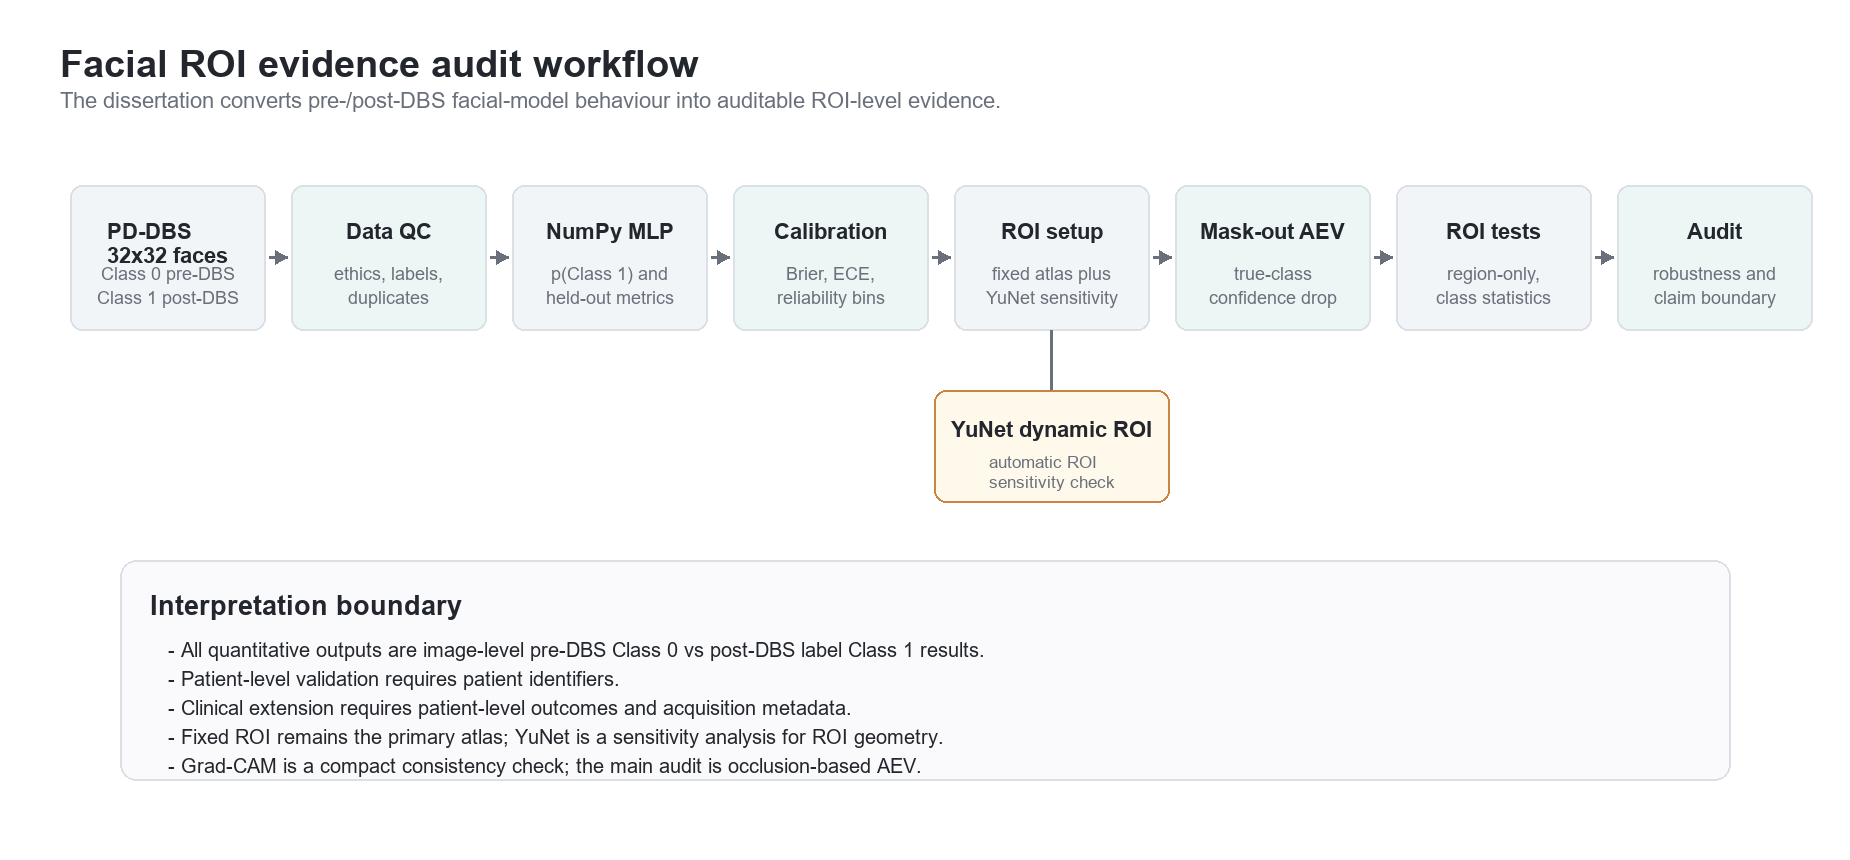
\includegraphics[width=0.98\textwidth]{figures/dissertation/fig_method_pipeline.png}
\caption{Facial ROI evidence audit workflow. The figure summarises the route from low-resolution PD-DBS facial images to pre-/post-DBS label classification, calibration, fixed and dynamic ROI definition, mask-out AEV, region-only validation, robustness checks, and explicit reporting scope.}
\end{figure}

The project used the local PD-DBS facial image file \path{data/raw/PD_DBS_Data.mat}. The file is a MATLAB 5.0 \path{.mat} file containing \texttt{\detokenize{x_train}}, \texttt{\detokenize{x_test}}, \texttt{\detokenize{y_train}}, and \texttt{\detokenize{y_test}}. It contains 2343 images in total: 1172 training images and 1171 test images.


The working file contained the image arrays and labels used for this study. Source-cohort details, acquisition protocol, original image resolution, down-sampling history, site or session variables, subject identifiers, and session identifiers were outside the provided metadata record. These fields were documented as study-scope variables and excluded from imputation.


Project ethics was approved by email after review of the submitted ethics form on 9 June 2026; the approval recorded that the dataset had already been authorised for research use.


Each image is represented as a 1024-dimensional vector corresponding to a 32$\times$32 grayscale image. Labels are encoded as 0/1 values under the project convention that Class 0 denotes pre-DBS and Class 1 denotes the supplied post-DBS label. All experiments therefore use the supplied pre-/post-DBS label task.


The provided record is image-level. The original train/test split was preserved to avoid introducing a new random split across all 2343 images. The supplied split is the reporting unit for all image-level experiments.


The task is therefore defined as a numeric binary classification problem. The classifier predicts the probability of Class 1, denoted \texttt{\detokenize{p_class1}}. The complementary probability for Class 0 is \texttt{\detokenize{1 - p_class1}}. This convention is used throughout baseline evaluation, calibration, occlusion, and AEV statistics.


\section{Data Loading and Quality Control (QC)}

A dedicated MATLAB 5 reader was implemented to keep data loading explicit and dependency-light. The loader extracts the four arrays, checks array dimensions, converts vectors to 32$\times$32 grayscale images, and preserves the original split. A contact sheet was generated to confirm that reconstructed images were visually interpretable as faces.


The raw image vectors were reshaped into 32$\times$32 images using the orientation chosen to match the visual structure observed in the original data-loading workflow. The reconstructed samples were inspected as a smoke test because an incorrect reshape order can transpose or distort faces.


The data QC stage recorded five key properties: total image count, split size, label counts, image resolution, and available metadata. These fields determine the reporting scope for the image-level pre-/post-DBS label experiments and explanation audits.


\section{Baseline Classification}

A compact NumPy multilayer perceptron (MLP) was used as the locked audit baseline to keep preprocessing, model fitting, prediction export, and downstream perturbation analysis reproducible within a small dependency footprint. A compact convolutional neural network (CNN) was trained separately as a secondary image model for architecture-sensitivity and Grad-CAM analysis.


The baseline uses per-feature z-score normalization fitted on the training subset, one hidden ReLU layer, a sigmoid Class 1 output, binary cross-entropy loss, and Adam-style optimization \boxcite{goodfellow2016deeplearning} \boxcite{kingma2015adam}. The original training set was split into training and validation subsets using stratification. The original test set was retained for final evaluation.


\begin{table}[htbp]
\centering
\scriptsize
\caption{NumPy MLP baseline specification}
\begin{tabularx}{\textwidth}{>{\raggedright\arraybackslash}X>{\raggedright\arraybackslash}X}
\toprule
Component & Specification \\
\midrule
Input & 1024 z-scored pixel values from each 32$\times$32 image \\
Architecture & One hidden ReLU layer with 64 units. Sigmoid Class 1 output \\
Loss and optimiser & Binary cross-entropy with Adam-style updates \\
Training protocol & Stratified 80/20 train/validation split within the supplied training set \\
Epochs and batch size & 300 epochs. Batch size 64 \\
Learning rate and L2 penalty & 0.001 learning rate. 0.0001 L2 penalty \\
Decision threshold & 0.5 on \texttt{\detokenize{p_class1}} for threshold metrics \\
Locked seed & 42 for the final headline run \\
\bottomrule
\end{tabularx}
\end{table}


Outputs use the fields \texttt{\detokenize{y_true}}, \texttt{\detokenize{p_class1}}, and \texttt{\detokenize{y_pred}}. The Class 1 probability is the supplied post-DBS label probability.


The locked MLP provides the saved probability outputs used for AEV, calibration, low-level, and region-only analyses. The compact CNN provides a second image-model check and the convolutional feature maps used for Grad-CAM.


Training used standard binary classification logic. The model was fitted on the training subset, monitored on a validation subset, and evaluated once on the held-out test split. Standardization parameters were fitted only from the training data and then applied to validation and test data. This avoids using test information during preprocessing. The final outputs include per-sample predictions so that later analyses can reuse the same probability values and avoid ad hoc retraining.


The evaluation metrics cover threshold-dependent and threshold-independent behaviour. Accuracy and F1 summarise performance at a classification threshold. Balanced accuracy accounts for class imbalance \boxcite{brodersen2010balanced}. AUROC assesses rank discrimination across thresholds \boxcite{fawcett2006roc}. Trapezoidal AUPRC summarises precision-recall behaviour when class proportions differ \boxcite{davis2006prroc} \boxcite{saito2015precision}. The majority-class baseline gives a simple reference for the imbalanced test set.


\section{Duplicate and Leakage QC}

Exact train-test duplicates were checked by hashing raw 1024-dimensional image vectors. Near-duplicate checks used nearest-train mean squared error (MSE) and maximum cosine similarity for each test image. This analysis can detect identical or highly similar images.


A second sensitivity analysis removed the flagged high-cosine near-duplicate test samples and recomputed key metrics. This check tests whether headline performance is dominated by a small number of duplicate or near-duplicate cases.


To assess broader similarity-related split sensitivity, an additional similarity-threshold analysis was added. The frozen test predictions were re-evaluated after excluding all test samples whose maximum cosine similarity to any training image exceeded progressively lower thresholds. This analysis is harsher than the original near-duplicate check because it removes broad similarity neighbourhoods.


Two low-level confound baselines were used. A global image-statistics baseline used eight non-anatomical summary features, including mean intensity, contrast, left-right mean difference, upper-lower mean difference, centre-border difference, and bright/dark pixel fractions. A per-ROI low-level baseline used five summary features per ROI: mean intensity, standard deviation, 10th percentile, 90th percentile, and mean gradient magnitude. These baselines assess how much label signal can be recovered from brightness, contrast, texture, and framing summaries without using the full pixel pattern.


The leakage and confound checks are therefore used as risk assessment. They document obvious duplicate leakage and provide context for the similarity-threshold and low-level baseline results.


\section{Calibration}

Calibration was evaluated from saved test-set predictions using Brier score and ECE with 10 equal-width bins over \texttt{\detokenize{p_class1}} \boxcite{brier1950verification} \boxcite{guo2017calibration}. Reliability-bin data were exported for later plotting.


The Brier score was computed as the mean squared error between predicted Class 1 probability and the numeric binary outcome. ECE was computed by assigning predictions to probability bins, calculating the absolute difference between mean confidence and observed Class 1 fraction in each bin, and taking the count-weighted average. Reliability-bin data were used to plot the observed Class 1 fraction against mean predicted probability.


The final reported calibration analysis uses the unscaled test-set probabilities from the locked baseline run \boxcite{guo2017calibration}. This documents the calibration context for the probability outputs used by AEV on the supplied pre-/post-DBS label task.


\section{Coarse Fixed-Atlas ROI Definition}

Eight mutually exclusive coarse named ROIs were defined on the 32$\times$32 image grid. The table below gives the intended facial-region scope and grid coverage for each region. Rows and columns use zero-indexed inclusive ranges. The machine-readable ROI names are stored in \path{outputs/roi/coarse_roi_definitions.csv}.


\begin{table}[htbp]
\centering
\scriptsize
\caption{Coarse fixed-atlas ROI definitions}
\begin{tabularx}{\textwidth}{>{\raggedright\arraybackslash}X>{\raggedright\arraybackslash}X>{\raggedright\arraybackslash}X>{\raggedright\arraybackslash}X>{\raggedright\arraybackslash}X}
\toprule
ROI & Anatomical coverage & Grid rows & Grid columns & Pixels \\
\midrule
Upper brow/forehead & Upper face, brow, forehead & 0-7 & 4-27 & 192 \\
Left periocular & Image-left periocular region & 8-14 & 0-13 & 98 \\
Right periocular & Image-right periocular region & 8-14 & 18-31 & 98 \\
Nasal midface & Nasal bridge and central midface & 8-21 & 14-17 & 56 \\
Left cheek/zygomatic & Image-left cheek and zygomatic region & 15-23 & 0-13 & 126 \\
Right cheek/zygomatic & Image-right cheek and zygomatic region & 15-23 & 18-31 & 126 \\
Perioral/mouth & Perioral and mouth region & 24-27 & 8-23 & 64 \\
Chin/mandible & Chin and mandible region & 28-31 & 6-25 & 80 \\
\bottomrule
\end{tabularx}
\end{table}

This coarse ROI design was used because the available image resolution supports broad region analysis. Standard facial landmark and face-localisation approaches assume substantially richer spatial detail than the present 32$\times$32 arrays provide \boxcite{kazemi2014one} \boxcite{zhang2016mtcnn} \boxcite{bulat2017far} \boxcite{deng2020retinaface}.


The ROI definitions were implemented as binary masks on the 32$\times$32 grid. Each mask identifies the pixels belonging to one named region. The masks were designed to be mutually exclusive, meaning that no pixel belongs to more than one ROI. This matters for interpretation: if ROIs overlap, evidence assigned to one region may partly duplicate evidence assigned to another. The final masks have zero overlapping pixels.


The fixed pixel-rectangle masks assume approximate face centring and similar framing. The provided record contained no landmark metadata, so centring was checked at a coarse level. Intensity-threshold foreground masks were used to estimate image centroids, bounding-box widths, bounding-box heights, and foreground fractions across train and test splits. This alignment QC summarises how the fixed-ROI layout matches the supplied 32$\times$32 images.


An automatic ROI-definition sensitivity analysis was added using OpenCV YuNet, a lightweight face detector designed for efficient face localisation \boxcite{wu2023yunet}. The original 32$\times$32 grayscale images were upsampled to 256$\times$256, YuNet detected the face and five coarse landmarks, and dynamic ROI boxes were derived to approximate the same eight ROI names. The primary AEV statistics used the fixed atlas so that every image shared one reproducible low-resolution coordinate system. YuNet was used to test how region-only and AEV results changed when ROI boxes followed detected face geometry.


\section{Occlusion-Based AEV}

For each test image and ROI, pixels inside the ROI were replaced by the corresponding training-set mean pixel values. The model then recomputed \texttt{\detokenize{p_class1}}.


True-class confidence was defined as:


\begin{verbatim}
true_confidence = p_class1       if y_true = 1
true_confidence = 1 - p_class1   if y_true = 0
\end{verbatim}

Occlusion evidence, reported as the true-class confidence drop, was defined as:


\begin{verbatim}
evidence_drop = true_confidence_original - true_confidence_masked
\end{verbatim}

Positive values indicate that masking the ROI reduced true-class confidence. The AEV for each image is the vector of true-class confidence drops across the eight ROIs.

\begin{figure}[H]
\centering
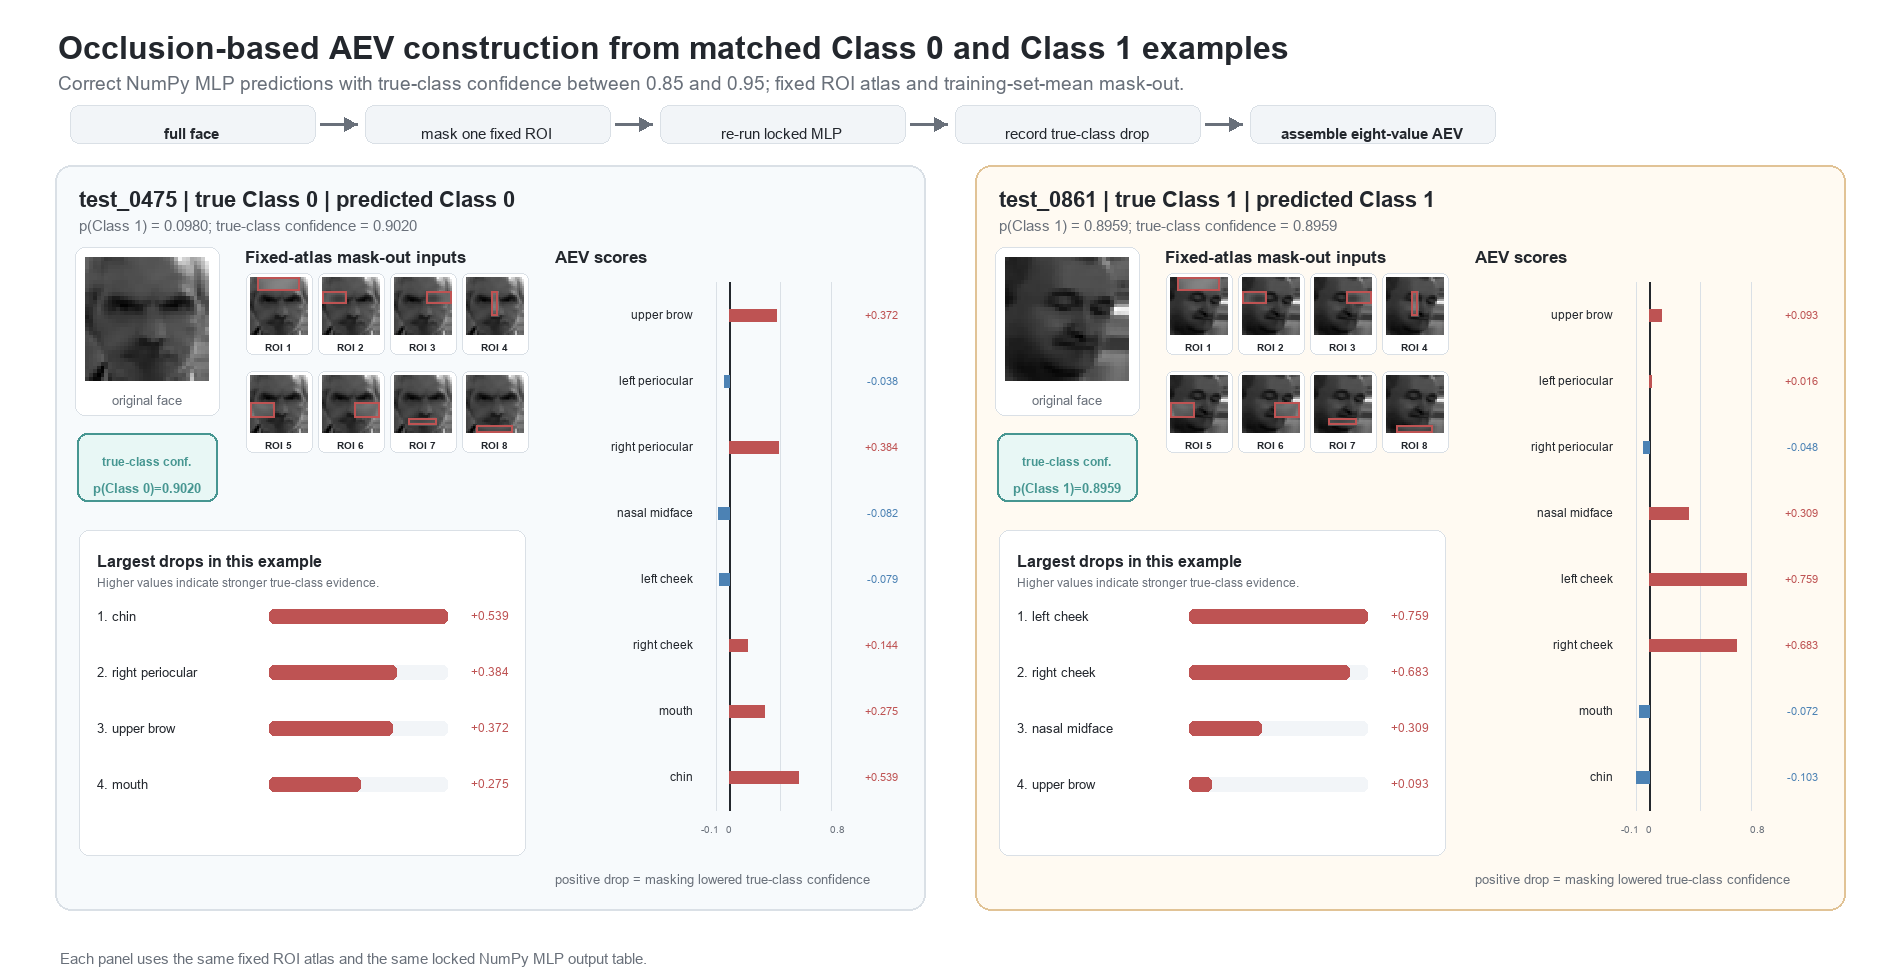
\includegraphics[width=\textwidth]{figures/dissertation/fig_aev_dual_worked_example.png}
\caption{Occlusion-based AEV construction for matched Class 0 and Class 1 test examples. Both examples are correct NumPy MLP predictions with true-class confidence between 0.85 and 0.95. For each sample, the figure shows the original 32$\times$32 face, eight fixed-atlas ROI mask-out inputs, and the resulting true-class confidence-drop vector.}
\end{figure}


The word anatomical is used operationally: it refers to the named coarse ROI coordinate system on the 32$\times$32 image grid. This convention keeps AEV scores tied to the implemented ROI layout.


Using the training-set mean as the replacement value avoids introducing an extreme artificial colour or intensity patch. It creates a neutralised version of the region relative to the learned training distribution. The perturbed image is still artificial, and attribution results can depend on the chosen baseline or reference value. The choice is a standard and transparent perturbation baseline for a low-resolution study \boxcite{zeiler2014visualizing} \boxcite{samek2017evaluating} \boxcite{sturmfels2020baselines}.


The use of true-class confidence is also deliberate. For correctly classified samples, true-class confidence and predicted-class confidence are usually the same. For misclassified samples, the two values differ. True-class drop measures how much masking a region reduces confidence in the ground-truth numeric label, including misclassified samples.


For each image, the final AEV is:


\begin{verbatim}
AEV_i = [drop_upper_brow_forehead, drop_left_periocular,
         drop_right_periocular, drop_nasal_midface,
         drop_left_cheek_zygomatic, drop_right_cheek_zygomatic,
         drop_perioral_mouth, drop_chin_mandible]
\end{verbatim}

Each component can be analysed per image, averaged across samples, compared between classes, or ranked within perturbation experiments.


\section{AEV Size Sensitivity}

Fixed-atlas mask-out scores were also summarised after dividing each ROI's mean true-class confidence drop by its pixel count. The normalized value was reported as confidence drop per 100 pixels:


\begin{verbatim}
drop_per_100_pixels = 100 * mean_evidence_drop / ROI_pixel_count
\end{verbatim}

This analysis checks how strongly raw full-region mask-out rankings track ROI size. Because raw mask-out drops scale with the number of masked pixels, cross-ROI comparisons of evidence intensity use the size-normalized score (confidence drop per 100 pixels) as the primary ranking lens. The raw AEV score is retained as the measure of the total effect of masking a complete named region. Both are reported so that total-region contribution and size-adjusted intensity can be read side by side.


\section{AEV Statistics}

Class 0 and Class 1 AEV distributions were compared ROI by ROI. The analysis computed class means and medians, mean difference, Cohen's d, Cliff's delta, permutation-test p-values, Benjamini-Hochberg FDR-adjusted p-values, and bootstrap 95\% confidence intervals \boxcite{cohen1988statistical} \boxcite{cliff1993dominance} \boxcite{benjamini1995controlling} \boxcite{efron1993bootstrap}.


The mean difference was defined as Class 1 mean evidence minus Class 0 mean evidence. A positive difference therefore indicates higher evidence in Class 1. A negative difference indicates higher evidence in Class 0. This convention is used consistently in the class-specific figures and tables.


Permutation testing was used because it makes fewer distributional assumptions than a parametric test \boxcite{good2005permutation}. For each ROI, class labels were repeatedly shuffled and the observed mean difference was compared against the null distribution of permuted differences. FDR correction was applied across the eight ROI tests to control false discovery rate. Effect sizes were reported because p-values alone leave the magnitude of regional evidence differences unspecified.


Bootstrap confidence intervals quantified uncertainty in the estimated mean differences.

The class-specific AEV analysis was run on the supplied test split used for the main fixed-split benchmark. The analysis used the same ROI masks, MLP probabilities, fill rule, confidence-drop definition, permutation testing, FDR correction, and bootstrap interval procedure for all eight ROIs.


\section{ROI Low-Level Confound Baseline}

The per-ROI low-level confound baseline was trained on 40 scalar features extracted from the same eight fixed ROIs. The feature set contained five summaries for each ROI: mean intensity, standard deviation, lower and upper intensity percentiles, and mean local gradient magnitude. The baseline used a standardised linear probabilistic classifier with the supplied train/test split.


This experiment tests whether broad ROI-local intensity and texture summaries carry label information. It uses summary-level regional features as a low-level comparator for AEV, raw-pixel modelling, and region-mask perturbation results.


\section{Pixel-Occlusion XAI Baseline}

As an additional explanation baseline, each pixel was occluded individually by replacing it with its training-set mean value. The true-class confidence drop for each pixel was then aggregated into the same eight fixed ROIs. This pixel-level baseline perturbs one pixel at a time before ROI aggregation. Region-mask AEV masks a complete region in one perturbation.


The pixel-occlusion baseline was compared with region-mask AEV using Spearman ROI-rank correlation and top-three ROI overlap. This provided a lightweight XAI comparator using the same trained MLP, test set, labels, fill value, and ROI atlas.


\section{Region-Only Validation}

For each ROI, pixels inside the ROI were retained and all other pixels were replaced with training-set mean values. The classifier then generated predictions from the region-only image. This measured retained-region response under the fixed MLP.


Region-only validation complements mask-out AEV. A high mask-out drop indicates that a region supports the full-face model in context. A high region-only AUROC indicates that the region alone contains information that can rank the numeric classes. Because facial evidence is likely distributed, region-only performance is expected to be lower than full-face performance. The key question is whether any region performs above chance or majority baseline.


The region-only experiment used the same trained MLP and the same test set. Differences across ROIs therefore reflect input perturbation under fixed model weights. Metrics were computed for each ROI separately, including accuracy, balanced accuracy, AUROC, trapezoidal AUPRC, and mean true-class confidence.


\section{Robustness}

Robustness analyses included near-duplicate sensitivity, five-seed training stability, mild blur perturbation, crop/resize perturbation, ROI evidence ranking stability under perturbation, fixed-ROI jitter, YuNet multi-seed checks, bootstrap fixed-versus-YuNet comparisons, label permutation, and occlusion fill-strategy sensitivity.


Multi-seed robustness was assessed across repeated random validation splits and model initialisations. This test captures variability from seed-dependent validation sampling and training, and the results are summarised as mean, standard deviation, and range across runs.


Perturbation robustness tested whether the trained model and the ROI evidence pattern were sensitive to small image changes, following the broader idea that vision models should be stress-tested under common corruptions and perturbations \boxcite{hendrycks2019robustness}. Mild blur approximates loss of sharpness. Centre crop and offset crop approximate spatial framing changes. At 32$\times$32 resolution, crop-based perturbations can shift or remove a large fraction of the face. For ROI evidence stability, rank correlation and top-3 overlap were used to assess whether high-evidence regions remained high under perturbation.


\section{Compact CNN and Grad-CAM Consistency Check}

The main audit pipeline used locked MLP probabilities for occlusion-based AEV, giving ROI-level evidence scores from one reproducible probability source. A compact PyTorch CNN was trained as a secondary image model for architecture-sensitivity and Grad-CAM analysis. Occlusion-based AEV uses forward passes through the MLP. Grad-CAM is computed from the CNN's convolutional feature maps. Cross-model agreement is reported as architecture-sensitivity evidence across model class and explanation mechanism. True-class Grad-CAM heatmaps were generated from the CNN and projected into the same eight fixed ROI masks used for occlusion \boxcite{zhou2016cam} \boxcite{selvaraju2017gradcam}.


Agreement was assessed at two levels. First, ROI-level Grad-CAM energy fractions were ranked against same-CNN ROI mask-out evidence drops using Spearman rank correlation and top-k ROI overlap. Second, a mean Grad-CAM map was compared with the ROI-weighted occlusion map using pixel top-k overlap. This check measures whether a gradient-based CNN explanation broadly supports the same regional evidence pattern as functional ROI occlusion.

Cross-model MLP-AEV/CNN-Grad-CAM comparisons were reported as sensitivity comparisons, with model architecture and explanation mechanism both changing.


\section{Controlled Comparison and Sensitivity Design}

The experiments were organised so that each comparison had a defined control structure. Same-model and same-split analyses were treated as controlled comparisons. Analyses that changed the split, ROI geometry, sample set, or model architecture were reported as sensitivity analyses, stress tests, or consistency checks.


\begin{table}[htbp]
\centering
\scriptsize
\caption{Controlled comparison design summary}
\begin{tabularx}{\textwidth}{>{\raggedright\arraybackslash}X>{\raggedright\arraybackslash}X>{\raggedright\arraybackslash}X>{\raggedright\arraybackslash}X}
\toprule
Experiment & Held constant & Changed or tested & Role in the audit \\
\midrule
Baseline MLP & Supplied train/test split, labels, preprocessing rule, threshold reporting & Learned numeric classifier & Establishes the predictive substrate for later explanation tests \\
Calibration & Saved MLP test predictions and supplied test labels & Probability bin and calibration metric & Checks whether confidence values used by AEV are numerically interpretable \\
Fixed-atlas mask-out AEV & MLP weights, test set, labels, fill value, eight fixed ROI names & Masked ROI & Controlled perturbation test of full-region contribution \\
Class-specific AEV statistics & Same AEV table, same test split, same ROI definitions & Class group comparison & Tests whether regional evidence differs between Class 0 and Class 1 \\
ROI low-level confound baseline & Same fixed ROI names and supplied split & ROI-local intensity and texture summaries & Assesses low-level regional confound signal without raw pixel-pattern modelling \\
Pixel-occlusion baseline & Same MLP, test set, labels, fill value, and ROI atlas & Pixel-wise occlusion followed by ROI aggregation & Provides a lightweight XAI comparator for region-mask AEV \\
Region-only validation & Same MLP, same test set, same fill value, same metric definitions & Retained ROI & Tests whether individual regions contain independent signal \\
Fixed atlas versus YuNet ROI & Same MLP, test set, labels, fill value, and ROI names & ROI geometry and pixel count & ROI-definition sensitivity analysis \\
Robustness checks & Frozen metrics or repeated training protocol, depending on test & Seed, blur, crop, fill value, label permutation, or ROI jitter & Stability and failure-mode assessment \\
Compact CNN / Grad-CAM & Same CNN, same test split, same true-class target & Explanation view and ROI projection & Secondary image-model and explanation-consistency check \\
\bottomrule
\end{tabularx}
\end{table}

This design assigns each result a defined evidential role. The main AEV and region-only analyses are controlled perturbation experiments under fixed model weights. YuNet and ROI jitter test sensitivity to ROI geometry. Low-level global and ROI baselines test brightness, texture, and framing signal. The reported values come from staged scripts and machine-readable outputs under \path{outputs/} and \path{models/}.



\chapter{Results}

Unless otherwise stated, Chapter 4 reports the supplied pre-/post-DBS image-level label task. Image-level metrics, ROI comparisons, calibration, and robustness checks are interpreted within that supplied-label setting.


\section{Dataset and Data Quality}
\begin{figure}[htbp]
\centering
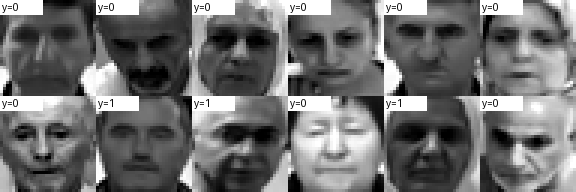
\includegraphics[width=0.72\textwidth]{figures/pd_dbs_smoke_samples.png}
\caption{PD-DBS data-loading smoke-test samples reconstructed from the local MATLAB file. The figure supports the data QC step and confirms that the 32$\times$32 grayscale inputs are visually interpretable as face images.}
\end{figure}
\begin{figure}[htbp]
\centering
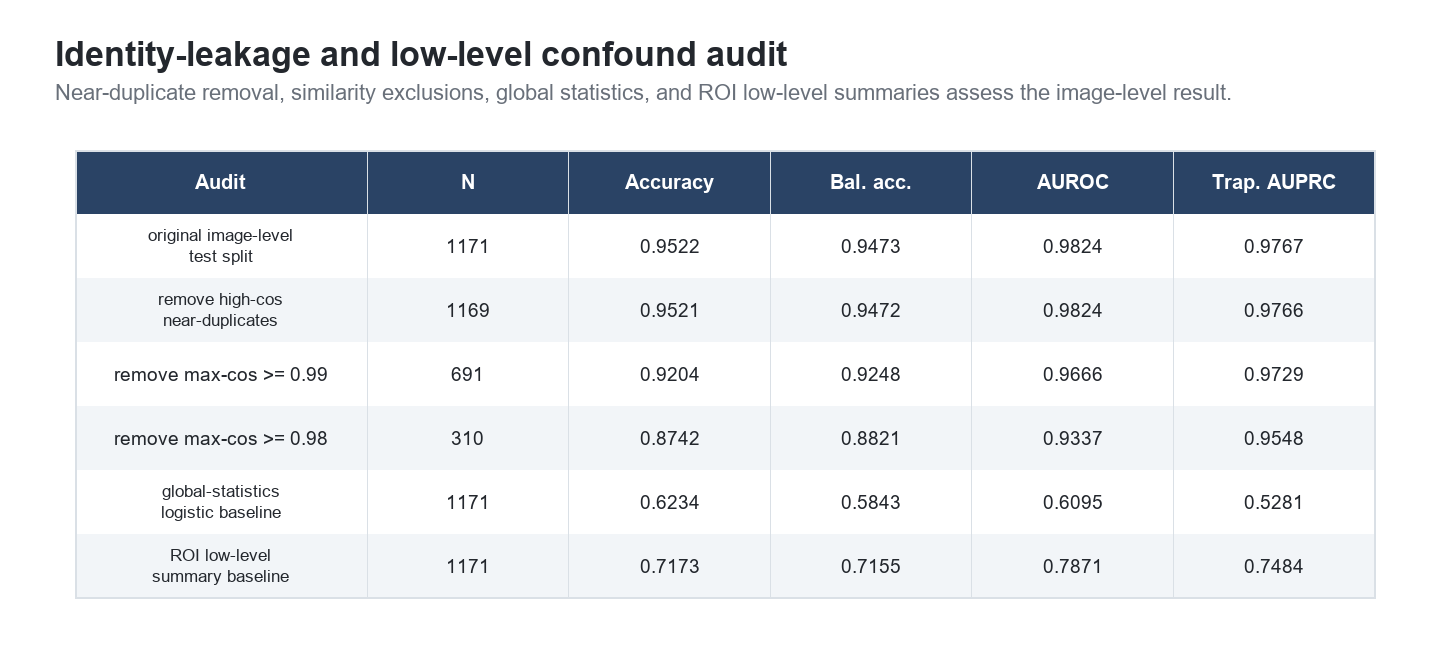
\includegraphics[width=0.95\textwidth]{figures/dissertation/fig_identity_leakage_audit.png}
\caption{Identity-leakage and low-level confound audit. The panel combines high-cosine near-duplicate removal, broader cosine-similarity exclusions, a global-statistics baseline, and an ROI low-level baseline for the supplied image-level test setting.}
\end{figure}

The dataset size, split, image resolution, and label convention are defined in Chapter 3. This section reports the corresponding QC and modelling results.


Duplicate QC found no exact train-test duplicate pairs and no near-duplicate pairs under MSE $\leq 10^{-5}$. Two high-cosine near-duplicate pairs were detected using cosine $\geq 0.999$. Removing these flagged samples left baseline metrics essentially unchanged.


The QC results confirm that the 32$\times$32 arrays are visually interpretable as facial images and can support a coarse ROI audit. The label-task evidence is evaluated through the classifier and audit analyses below.


Exact-duplicate QC found zero train-test duplicate pairs, addressing the simplest train-test leakage check. Subject-level leakage remains possible. Multiple images from the same person can differ enough to avoid exact or near-identical matching and still allow identity-like recognition. Broader similarity-based leakage and confound sensitivity were assessed beyond duplicate removal.


Progressively excluding test samples with high maximum cosine similarity to the training set reduced performance as the exclusion became stricter. Removing the two high-cosine cases left headline metrics essentially unchanged. Removing samples with max-cosine $\geq$ 0.99 left 691 test images and gave AUROC 0.9666. The max-cosine $\geq$ 0.98 rule left 310 test images and gave AUROC 0.9337. Broader similarity-threshold analyses therefore show some split sensitivity.


A global-statistics logistic baseline using eight brightness, contrast, and framing summaries achieved 0.6234 accuracy, 0.5843 balanced accuracy, and 0.6095 AUROC. The strongest single global-statistic/label correlation was upper-minus-lower mean intensity on the test split, r = -0.1429. A per-ROI low-level baseline using 40 intensity and texture summaries achieved 0.7173 accuracy, 0.7155 balanced accuracy, and 0.7871 AUROC. These results show substantial label-associated signal in low-level regional summaries.


Coarse alignment QC supported the fixed-ROI assumption at a broad level. Estimated intensity centroids were similar across train and test splits, with mean x-centroid 16.15 in train and 16.17 in test, and mean y-centroid 13.78 in train and 13.78 in test. Bounding boxes usually spanned most of the 32$\times$32 grid. This supports approximate centring and framing. The ROI analysis is therefore reported as coarse region evidence.


The 32$\times$32 resolution motivates both the validation scope and the coarse-ROI AEV design. The images are visually interpretable. The analysis therefore uses broad regions matched to the pixel grid.


\section{Baseline Pre-/Post-DBS Classification}

\begin{table}[htbp]
\centering
\scriptsize
\caption{Baseline NumPy MLP performance on the supplied image-level split. Under progressive similarity exclusion the headline AUROC of 0.9824 falls to 0.9666 (max-cosine $\geq$ 0.99, n = 691) and 0.9337 (max-cosine $\geq$ 0.98, n = 310). See Section 4.1.}
\begin{tabularx}{\textwidth}{>{\raggedright\arraybackslash}X>{\raggedright\arraybackslash}X}
\toprule
Metric & Value \\
\midrule
Majority baseline accuracy & 0.5764 \\
Accuracy & 0.9522 \\
Balanced accuracy & 0.9473 \\
F1 class 1 & 0.9419 \\
AUROC & 0.9824 \\
Trapezoidal AUPRC & 0.9767 \\
Brier score & 0.0402 \\
\bottomrule
\end{tabularx}
\end{table}

\begin{table}[htbp]
\centering
\scriptsize
\caption{Test-set confusion matrix}
\begin{tabularx}{\textwidth}{>{\raggedright\arraybackslash}X>{\raggedright\arraybackslash}X>{\raggedright\arraybackslash}X}
\toprule
 & Pred 0 & Pred 1 \\
\midrule
True 0 & 661 & 14 \\
True 1 & 42 & 454 \\
\bottomrule
\end{tabularx}
\end{table}
\begin{figure}[t]
\centering
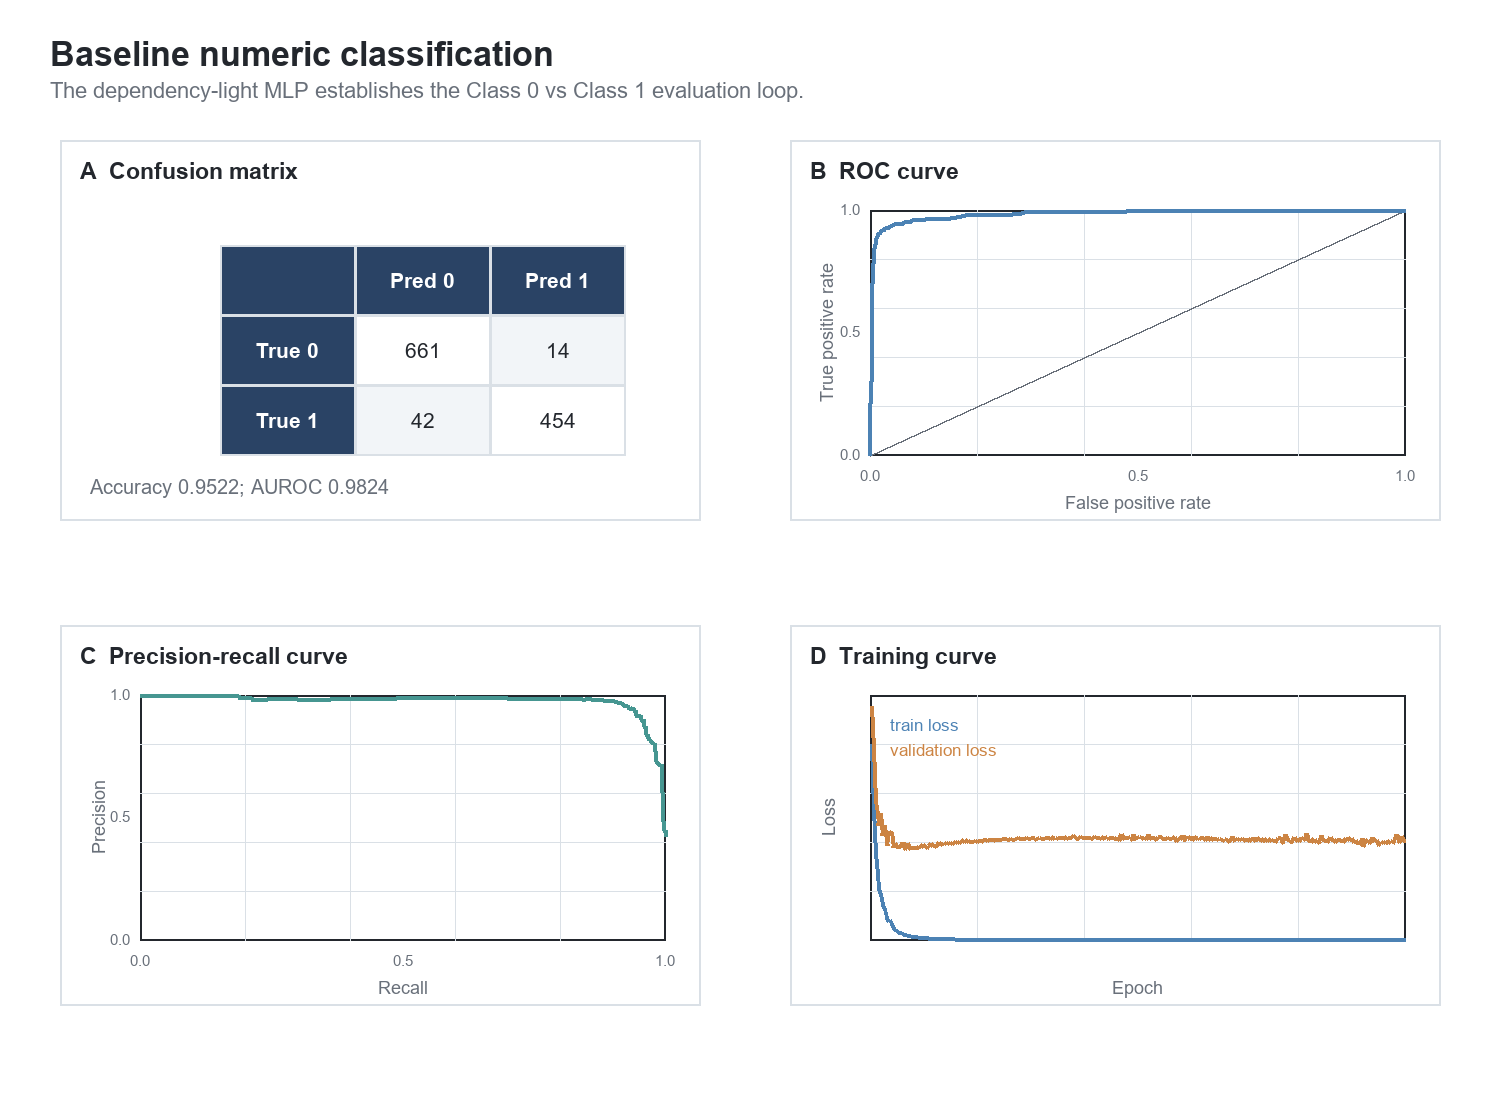
\includegraphics[width=1.00\textwidth]{figures/dissertation/fig_baseline_panel.png}
\caption{Baseline pre-/post-DBS evaluation. The panel summarises the confusion matrix, ROC curve, precision-recall curve and training curve for the dependency-light NumPy MLP baseline.}
\end{figure}

These results establish a strong supplied-split image-level baseline. A compact CNN secondary image model reached 0.9744 accuracy, 0.9727 balanced accuracy, and 0.9951 AUROC on the same supplied split. The CNN also captured the supplied split signal. The locked MLP provides the saved probabilities used for AEV, calibration, low-level, and region-only outputs. The 0.9824 AUROC is reported for the supplied image-level split.


The model substantially exceeded the majority-class baseline. The high balanced accuracy indicates strong performance on both numeric classes.


AUROC and AUPRC show strong ranking and precision-recall behaviour. At the selected threshold, the confusion matrix shows more missed Class 1 samples than incorrect Class 1 assignments for Class 0 samples. This threshold-specific behaviour describes the classifier on the supplied image-level split.


\section{Calibration}
The Brier score was 0.0402 and ECE with 10 equal-width bins was 0.0231. The mean predicted Class 1 probability was 0.4056, and the observed Class 1 fraction was 0.4236. These values indicate no gross miscalibration on the supplied pre-/post-DBS label task.


The reliability curve shows that the model's predicted probabilities broadly track observed Class 1 frequencies across bins. Because AEV is based on confidence change after perturbation, this calibration result supports the numerical use of confidence-drop scores.


In the following AEV analyses, confidence-drop scores use these same unscaled probabilities and supplied labels.

\begin{figure}[t]
\centering
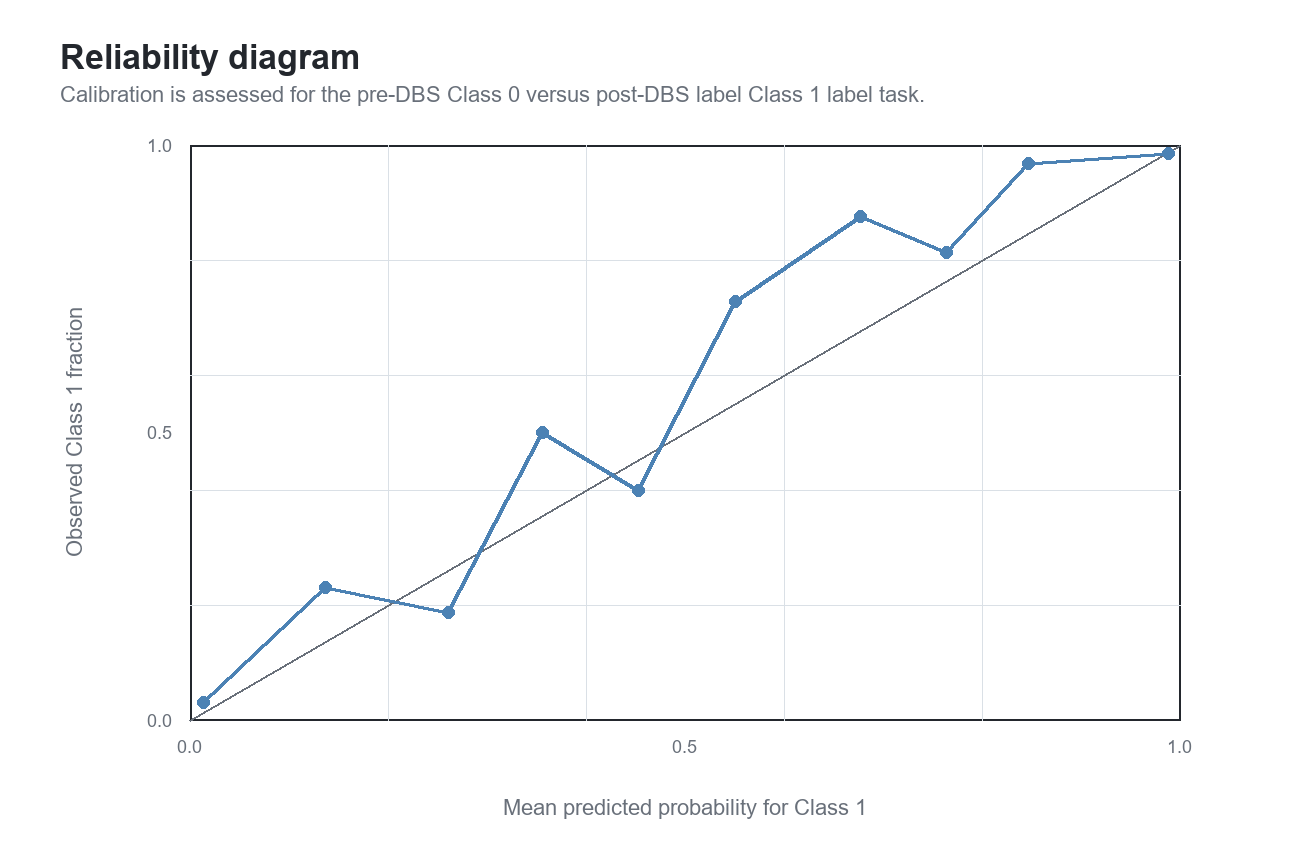
\includegraphics[width=0.66\textwidth]{figures/dissertation/fig_calibration_reliability.png}
\caption{Reliability diagram for the supplied pre-/post-DBS label task.}
\end{figure}


\section{Coarse ROI Design}
The implemented atlas used eight coarse fixed ROIs on the 32$\times$32 grayscale image grid. This scale matched the low-resolution setting.


The final ROI masks were mutually exclusive, with zero overlapping pixels. This avoided duplicated evidence around the cheek and mouth boundaries.


The eight ROIs cover 840 pixels of the 1024-pixel image grid. Unassigned pixels mainly include border and background areas, so the masks focus on interpretable facial regions.


The coarse ROI design is a fixed-region atlas for the available 32$\times$32 images. It demonstrates the AEV workflow in a low-resolution setting. A higher-resolution future dataset could support a more detailed craniofacial atlas with separate brow, orbital, nasal, philtrum, lip, chin, mandibular, and cheek regions.

\begin{figure}[H]
\centering
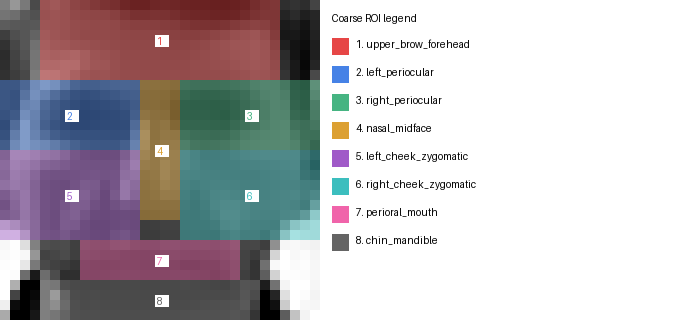
\includegraphics[width=0.62\textwidth]{outputs/roi/coarse_roi_overlay_examples.png}
\caption{Mutually exclusive coarse ROI overlay for the 32$\times$32 image grid. The low-resolution ROI design uses broad facial regions matched to the available image detail.}
\end{figure}


\section{Occlusion-Based AEV}
\begin{figure}[htbp]
\centering
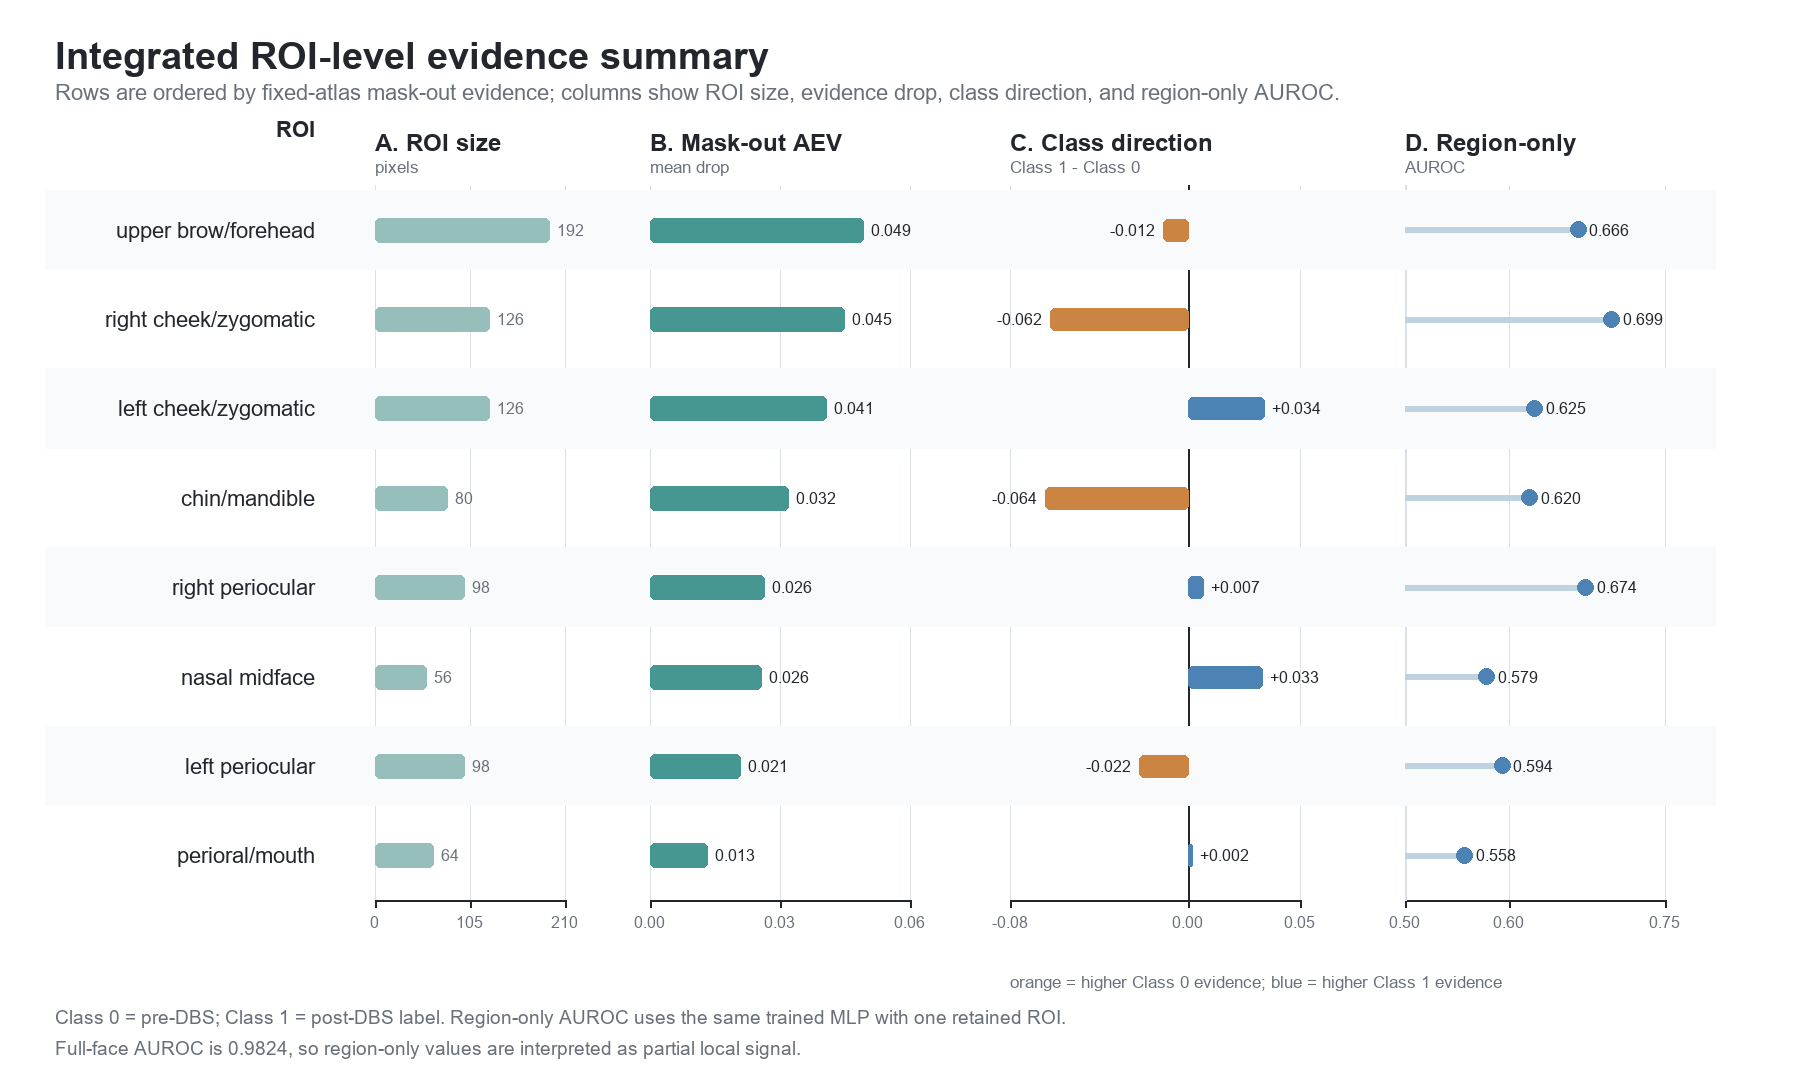
\includegraphics[width=0.98\textwidth]{figures/dissertation/fig_roi_evidence_summary.png}
\caption{Integrated ROI-level evidence summary. Rows are ordered by fixed-atlas mask-out AEV. Columns show ROI size, mean true-class confidence drop, Class 1 minus Class 0 evidence difference, and same-MLP region-only AUROC.}
\end{figure}

\begin{table}[htbp]
\centering
\scriptsize
\caption{Largest raw mean true-class confidence drops under fixed-atlas ROI mask-out}
\begin{tabularx}{\textwidth}{>{\raggedright\arraybackslash}X>{\raggedright\arraybackslash}X}
\toprule
ROI & Mean evidence drop \\
\midrule
\texttt{\detokenize{upper_brow_forehead}} & 0.049135 \\
\texttt{\detokenize{right_cheek_zygomatic}} & 0.044752 \\
\texttt{\detokenize{left_cheek_zygomatic}} & 0.040594 \\
\texttt{\detokenize{chin_mandible}} & 0.031842 \\
\bottomrule
\end{tabularx}
\end{table}

These ROIs produced the largest raw reductions in true-class confidence under mask-out testing, indicating that masking them had the strongest complete-region effect on the model's confidence in the true numeric class.


Raw full-region AEV scores were strongly associated with ROI size. Across the eight fixed ROIs, Pearson correlation between ROI pixel count and raw mean drop was 0.8307, and Spearman rank correlation was 0.8073. This means that the raw ranking is best read as total perturbation effect for a complete named region.


\begin{table}[htbp]
\centering
\scriptsize
\caption{Fixed-atlas AEV size-normalized sensitivity summary}
\begin{tabularx}{\textwidth}{>{\raggedright\arraybackslash}X>{\raggedright\arraybackslash}X>{\raggedright\arraybackslash}X>{\raggedright\arraybackslash}X>{\raggedright\arraybackslash}X}
\toprule
ROI & Pixels & Raw mean drop & Raw rank & Drop per 100 pixels / rank \\
\midrule
Nasal midface & 56 & 0.025674 & 6 & 0.045846 / 1 \\
Chin/mandible & 80 & 0.031842 & 4 & 0.039802 / 2 \\
Right cheek/zygomatic & 126 & 0.044752 & 2 & 0.035518 / 3 \\
Left cheek/zygomatic & 126 & 0.040594 & 3 & 0.032218 / 4 \\
Right periocular & 98 & 0.026388 & 5 & 0.026927 / 5 \\
Upper brow/forehead & 192 & 0.049135 & 1 & 0.025591 / 6 \\
Left periocular & 98 & 0.020829 & 7 & 0.021254 / 7 \\
Perioral/mouth & 64 & 0.013141 & 8 & 0.020534 / 8 \\
\bottomrule
\end{tabularx}
\end{table}


The size-normalized sensitivity check changed the ranking. Nasal midface and chin/mandible moved upward after dividing by pixel count. Upper brow/forehead moved from the highest raw mean drop to sixth by drop per 100 pixels. The perioral/mouth region stayed lowest in both summaries.


Evidence-drop values are true-class confidence changes after region masking. A high evidence drop means that replacing a region with training-set mean values reduced the classifier's confidence in the true numeric label.


The raw and normalized summaries therefore answer different measurement questions. Raw AEV reports the total effect of masking a full ROI. The size-normalized ranking is the primary lens for comparing evidence intensity across ROIs of different sizes, because raw drops scale with ROI pixel count. Region-only validation, YuNet sensitivity, and perturbation tests provide additional context for these fixed-ROI measurements.


\section{Class-Specific AEV Statistics}

\begin{table}[htbp]
\centering
\scriptsize
\caption{Fixed-atlas AEV class-specific statistics on the supplied split}
\begin{tabularx}{\textwidth}{>{\raggedright\arraybackslash}X>{\raggedright\arraybackslash}X>{\raggedright\arraybackslash}X>{\raggedright\arraybackslash}X>{\raggedright\arraybackslash}X>{\raggedright\arraybackslash}X}
\toprule
ROI & Direction & Difference [95\% CI] & Cohen d & Cliff delta & FDR \\
\midrule
Chin/mandible & higher in Class 0 & -0.0645 [-0.0795, -0.0496] & -0.4792 & -0.3397 & 0.0005 \\
Right cheek/zygomatic & higher in Class 0 & -0.0622 [-0.0805, -0.0440] & -0.3786 & -0.2943 & 0.0005 \\
Left cheek/zygomatic & higher in Class 1 & 0.0340 [0.0125, 0.0556] & 0.1953 & 0.0111 & 0.0022 \\
Nasal midface & higher in Class 1 & 0.0328 [0.0189, 0.0480] & 0.2769 & 0.1885 & 0.0005 \\
Left periocular & higher in Class 0 & -0.0223 [-0.0352, -0.0098] & -0.2048 & -0.2049 & 0.0022 \\
Upper brow/forehead & higher in Class 0 & -0.0116 [-0.0307, 0.0081] & -0.0711 & 0.0047 & 0.3026 \\
Right periocular & higher in Class 1 & 0.0067 [-0.0068, 0.0202] & 0.0587 & 0.1259 & 0.3709 \\
Perioral/mouth & higher in Class 1 & 0.0017 [-0.0100, 0.0131] & 0.0189 & -0.1252 & 0.7544 \\
\bottomrule
\end{tabularx}
\end{table}

Class-specific analysis adds directionality to the global importance ranking. Chin/mandible, right cheek/zygomatic, and left periocular evidence were higher in Class 0. Left cheek/zygomatic and nasal midface evidence were higher in Class 1. The difference is defined as Class 1 minus Class 0. Negative values indicate higher pre-DBS evidence, and positive values indicate higher supplied post-DBS label evidence. Five ROIs remained significant after FDR correction. The remaining three ROIs are reported as non-significant supplied-split estimates.


Together, the supplied-split class statistics show how AEV turns explanation into an auditable statistical object. Regional evidence can be ranked, tested, assigned effect sizes, and checked with confidence intervals. The reported AEV directions are supplied-split findings and are read alongside the low-level confound baselines.


\section{Region-Only Validation}
The best region-only ROI was \texttt{\detokenize{right_cheek_zygomatic}}, with 0.6763 accuracy, 0.6551 balanced accuracy, and 0.6988 AUROC. Region-only validation tests the fixed MLP response when one ROI is retained. The best retained-region response was lower than the full-face AUROC of 0.9824 and the ROI low-level summary baseline AUROC of 0.7871. Simple regional intensity and texture summaries carried stronger label-ranking signal than any single retained fixed ROI.


The right cheek/zygomatic region ranked highest in region-only validation and also appeared among the strongest raw occlusion regions. This agreement identifies a stable retained-region response for the supplied label task. The gap between region-only, low-level ROI baseline, and full-face performance is an audit finding. AEV records how the trained model responds to named-region perturbations, and the low-level baseline quantifies regional intensity and texture signal.


As an automatic ROI-definition sensitivity check, YuNet was run after upsampling the 32$\times$32 images to 256$\times$256. YuNet detected all 2343 faces. The main region-only comparison tested whether the fixed-atlas right-cheek signal persisted under automatically defined ROI boxes.

\begin{figure}[t]
\centering
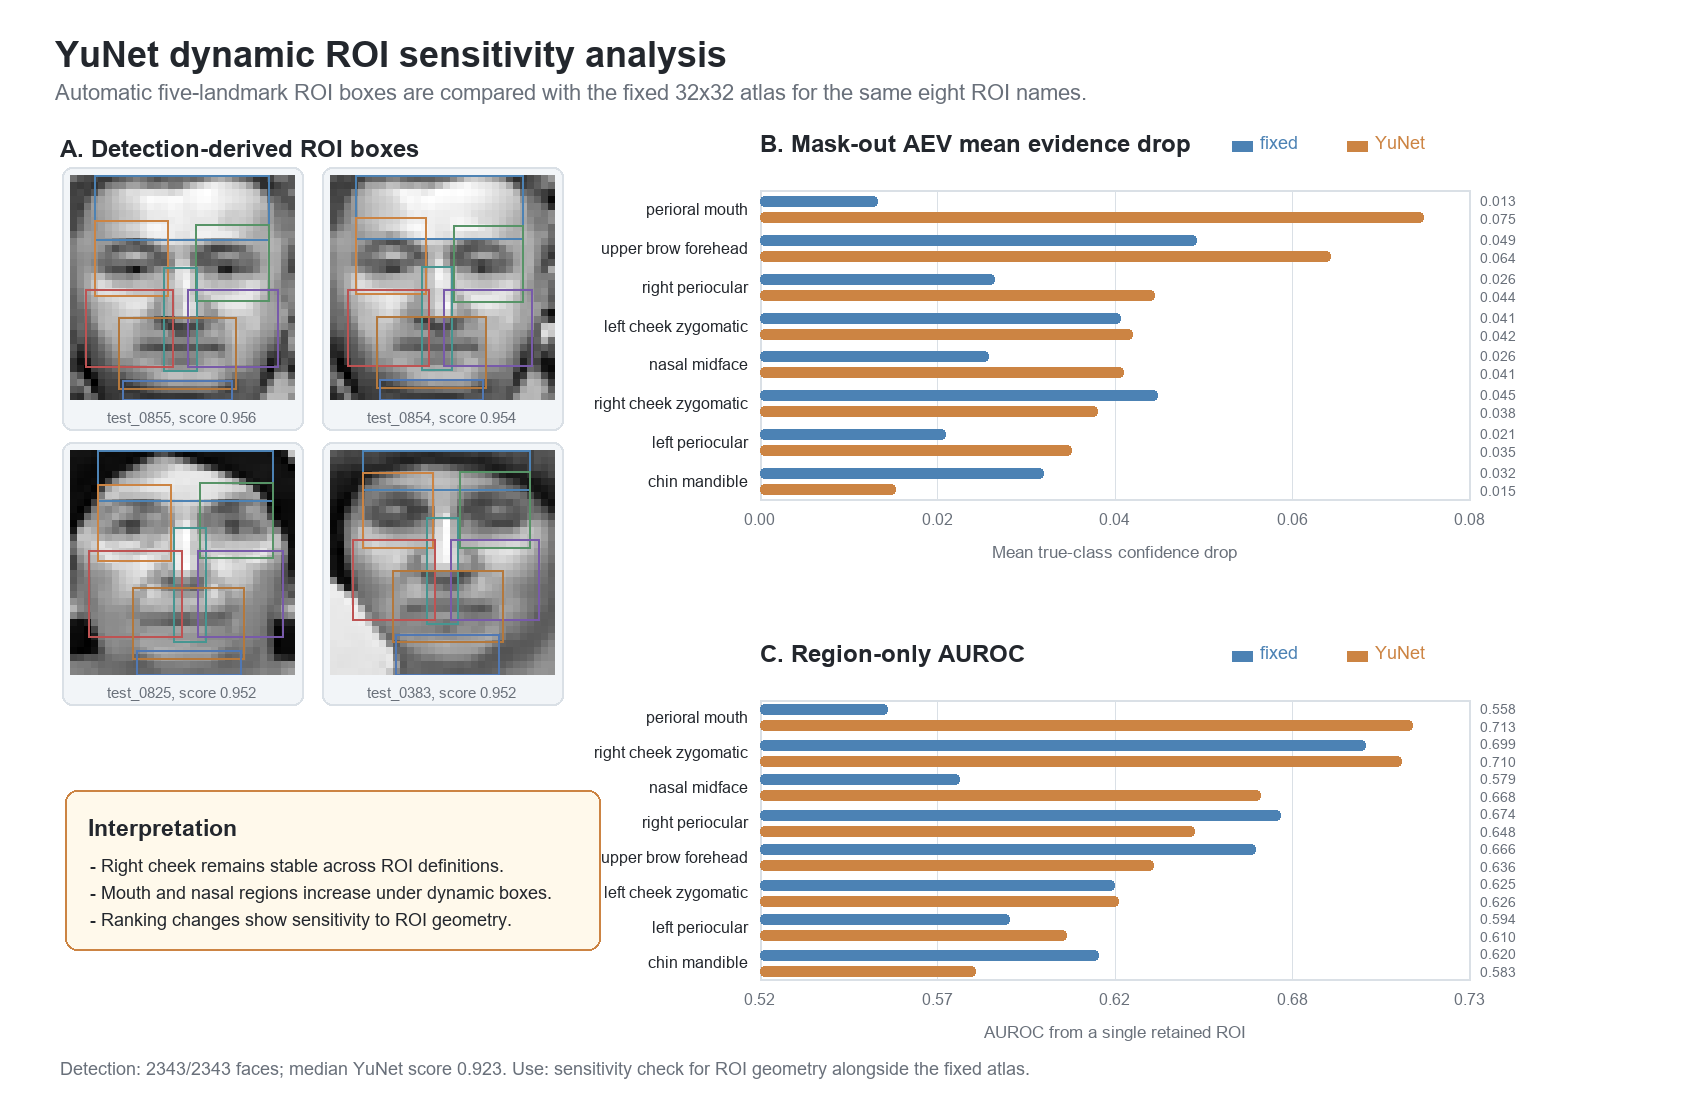
\includegraphics[width=1.00\textwidth]{figures/dissertation/fig_yunet_dynamic_roi_sensitivity.png}
\caption{YuNet dynamic ROI sensitivity analysis. Automatic five-landmark ROI boxes are compared with the fixed 32$\times$32 atlas for detection-derived ROI examples, mask-out AEV mean evidence drops, and region-only AUROC. The comparison tests ROI-geometry sensitivity.}
\end{figure}


\begin{table}[htbp]
\centering
\scriptsize
\caption{Fixed-atlas versus YuNet-derived region-only validation}
\begin{tabularx}{\textwidth}{>{\raggedright\arraybackslash}X>{\raggedright\arraybackslash}X>{\raggedright\arraybackslash}X>{\raggedright\arraybackslash}X>{\raggedright\arraybackslash}X>{\raggedright\arraybackslash}X>{\raggedright\arraybackslash}X}
\toprule
ROI & Fixed BA & Fixed AUROC & YuNet BA & YuNet AUROC & Delta BA & Delta AUROC \\
\midrule
Right cheek & 0.6551 & 0.6988 & 0.6575 & 0.7096 & 0.0024 & 0.0107 \\
Mouth & 0.5560 & 0.5577 & 0.6535 & 0.7129 & 0.0975 & 0.1552 \\
Nasal midface & 0.5548 & 0.5788 & 0.6248 & 0.6679 & 0.0700 & 0.0891 \\
\bottomrule
\end{tabularx}
\end{table}

These fixed-versus-YuNet deltas measure ROI-definition sensitivity. The model, test set, labels, fill value, and ROI names are held fixed. ROI geometry and pixel count change together when YuNet boxes replace the fixed atlas.


For right cheek/zygomatic, the YuNet-minus-fixed AUROC difference was small: delta 0.0107 with a 95\% bootstrap interval from -0.0200 to 0.0417. The balanced-accuracy delta was 0.0024 with a 95\% bootstrap interval from -0.0291 to 0.0348. A fixed-ROI jitter test gave the same top region in 10 of 11 atlas variants, and the right-cheek AUROC range across jittered variants was 0.6896 to 0.7197. These checks support the right-cheek region-only result as spatially stable under small ROI-definition changes.


YuNet dynamic AEV gave a different ranking from the fixed-atlas AEV. The largest YuNet evidence drops were perioral/mouth 0.0747, upper brow/forehead 0.0642, and right periocular 0.0444. Right cheek/zygomatic remained measurable at 0.0380. The shift is an ROI-geometry sensitivity finding. Fixed rectangular masks and detection-derived boxes capture different pixel areas, especially around the mouth. The fixed atlas is used as the primary AEV system because it gives one reproducible 32$\times$32 coordinate frame for class statistics, occlusion, region-only validation, and robustness checks.


\section{Low-Level / Full-Pixel Score Decomposition}

To examine how the full-pixel MLP score related to low-level regional image summaries, an exploratory block-wise logistic decomposition was conducted on the supplied test split. The decomposition model used five-fold out-of-fold (OOF) cross-validation within the test split. The analysis compares the incremental ranking discrimination of two fixed predictor blocks under one common audit protocol.

Under this protocol, the 40 ROI low-level summary features alone reached an out-of-fold AUROC of 0.7709, and the locked full-pixel MLP score alone reached 0.9794. Combining the two blocks gave 0.9752. Adding the full-pixel score to the low-level block increased AUROC by +0.2043. Adding the low-level block to the full-pixel score changed AUROC by -0.0042. All three values use the same out-of-fold protocol. The separately reported headline AUROC of 0.9824 (Table 4.7) is the locked model's train-to-test score. This asymmetric pattern shows that low-level ROI summaries carry measurable label-associated signal and add no ranking discrimination beyond the full-pixel MLP score in this decomposition.

The decomposition supports a two-part interpretation. First, ROI-level brightness and texture summaries contain substantial label-associated information. Second, the full-pixel MLP score captures additional split-specific structure beyond these 40 summaries. Attribution of that additional structure to facial morphology, DBS state, identity, or acquisition effects is a later patient-level analysis using identity and acquisition metadata.


\begin{table}[htbp]
\centering
\scriptsize
\caption{Low-level / full-pixel score decomposition on the supplied test split. The upper block lists the headline baselines fitted on the training split and evaluated on the test split (Section 4.1). The lower block is an exploratory five-fold out-of-fold (OOF) logistic decomposition computed within the test split. All OOF rows share one protocol and are directly comparable. The train-to-test headline AUROC is reported as a reference anchor.}
\begin{tabularx}{\textwidth}{>{\raggedright\arraybackslash}X>{\raggedright\arraybackslash}X}
\toprule
Predictor & AUROC \\
\midrule
\multicolumn{2}{l}{\textit{Headline baselines (train$\rightarrow$test fit, Section 4.1)}} \\
Majority baseline & 0.500 \\
Global image-statistics confound (8 features) & 0.6095 \\
ROI low-level confound (40 features) & 0.7871 \\
Full-pixel MLP & 0.982 \\
\midrule
\multicolumn{2}{l}{\textit{Exploratory decomposition (5-fold out-of-fold logistic, test split)}} \\
ROI low-level summaries only & 0.7709 \\
Full-pixel MLP score only & 0.9794 \\
Low-level summaries + full-pixel MLP score & 0.9752 \\
Increment of MLP score over low-level & +0.2043 \\
Increment of low-level over MLP score & -0.0042 \\
\bottomrule
\end{tabularx}
\end{table}


\section{Robustness}
\begin{figure}[htbp]
\centering
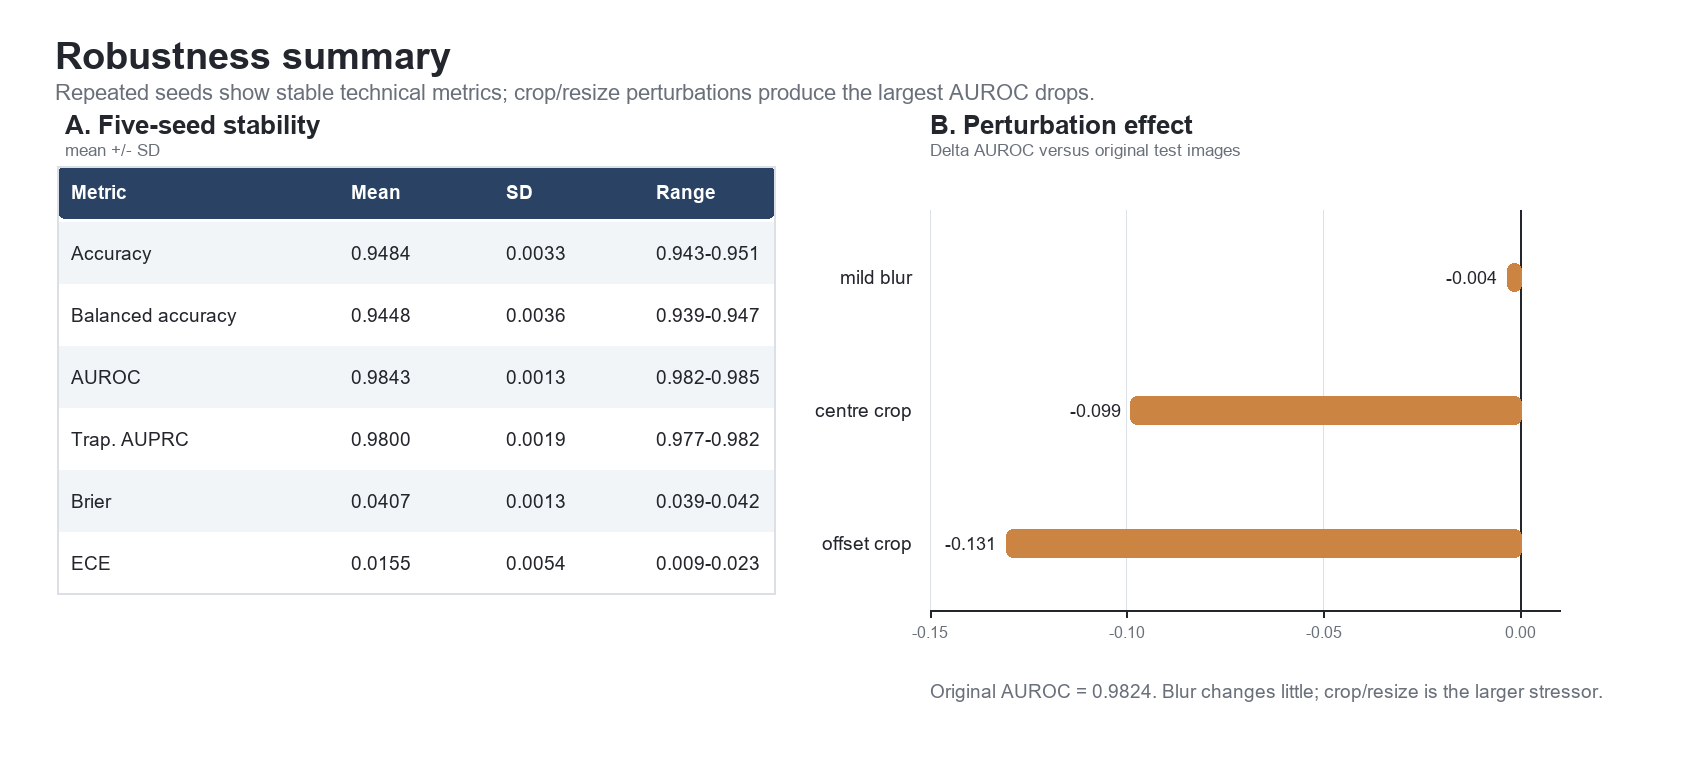
\includegraphics[width=0.98\textwidth]{figures/dissertation/fig_robustness_summary.png}
\caption{Robustness summary. Multi-seed stability is reported as mean, standard deviation, and range across repeated runs. Perturbation robustness is reported as AUROC change relative to original test images.}
\end{figure}

The headline AUROC of 0.9824 comes from the locked final run. The multi-seed values in Figure 4.8 are means across repeated validation splits and model initialisations.


The multi-seed results show stable baseline behaviour across random seeds. Accuracy, balanced accuracy, AUROC, and trapezoidal AUPRC all had small standard deviations across repeated splits and initialisations. This supports the stability of the pre-/post-DBS label classification pipeline.


The perturbation results show a more specific pattern. Mild blur had very limited effect on AUROC, with AUROC delta -0.0035 and ROI rank correlation 0.9762 with top-3 overlap of 3/3. In contrast, centre crop and offset crop reduced AUROC more substantially, with deltas of -0.0991 and -0.1307. This is expected in 32$\times$32 facial images because cropping can shift or remove a large portion of the face.


Additional ROI sensitivity checks refined the robustness picture. Label permutation reduced full-face AUROC to a near-chance mean of 0.5450 across three seeds. Occlusion fill-strategy analysis showed that zero fill produced large out-of-distribution effects. Blur fill produced very small evidence drops and unstable rankings. Training-mean fill was therefore retained for the main AEV analysis. In the MLP region-only sensitivity outputs, fixed-versus-YuNet rank correlation was weak across all eight ROIs, and the fixed and YuNet analyses agreed on right cheek/zygomatic as the top balanced-accuracy region.


\section{Compact CNN and Grad-CAM ROI Agreement}
A compact CNN was trained as a secondary image model and Grad-CAM source. On the supplied image-level split it achieved 0.9744 accuracy, 0.9727 balanced accuracy, and 0.9951 AUROC. Two independent ROI-rank comparisons gave Spearman rho = 0.9524: Grad-CAM projection versus same-CNN fixed-atlas occlusion, and same-CNN fixed-atlas occlusion versus same-CNN YuNet automatic-ROI occlusion. In both comparisons, the top-three ROI overlap was 3/3.


The 0.9524 correlations are same-CNN sanity checks: two explanation views of the compact CNN ranked the fixed ROIs similarly. Cross-model comparisons change both architecture and explanation mechanism. MLP region-mask AEV versus CNN Grad-CAM gave Spearman rho = 0.7857, and MLP region-mask AEV versus pixel-occlusion ROI aggregation gave rho = 0.3810 and 0.6429.


\begin{figure}[H]
\centering
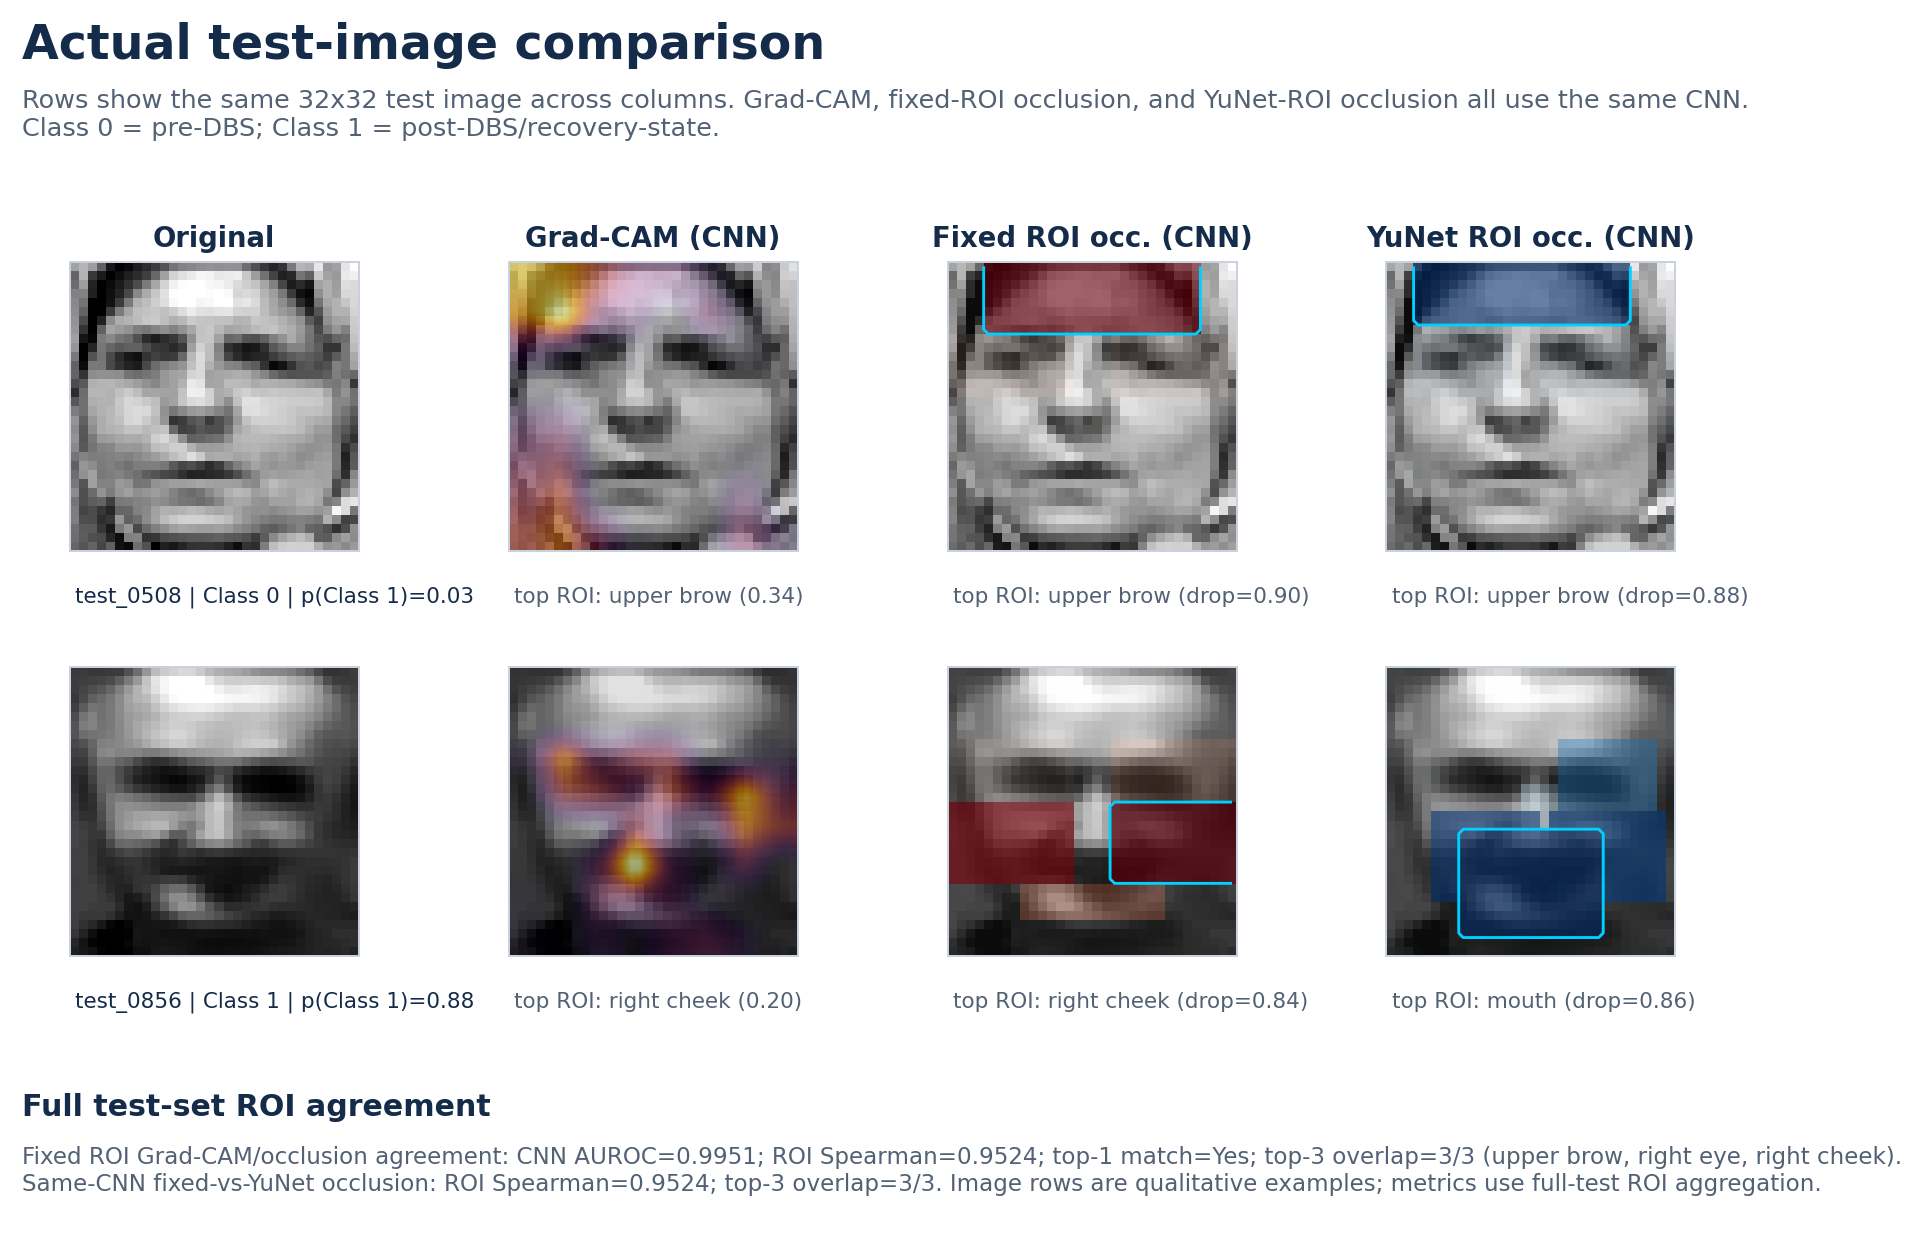
\includegraphics[width=1.00\textwidth]{figures/dissertation/fig_gradcam_occlusion_overlap.png}
\caption{Grad-CAM and ROI occlusion comparison on real test images. Each row shows the same 32$\times$32 test image as the original input, CNN Grad-CAM, CNN fixed-atlas ROI occlusion, and CNN YuNet automatic-ROI occlusion. The quantitative comparison is based on full test-set ROI aggregation.}
\end{figure}

The pixel-occlusion baseline provides a lighter perturbation comparator: each pixel was masked individually and then aggregated into the same eight ROIs. Its agreement with region-mask AEV was moderate when pixel drops were summed within ROIs. Cross-model agreement between MLP AEV and CNN Grad-CAM was moderate-to-high at ROI rank level. Same-CNN Grad-CAM versus same-CNN occlusion remained the strongest agreement.

\begin{table}[H]
\centering
\scriptsize
\caption{XAI baseline and cross-method ROI-rank comparisons}
\begin{tabularx}{\textwidth}{>{\raggedright\arraybackslash}X>{\raggedright\arraybackslash}X>{\raggedright\arraybackslash}X}
\toprule
Comparison & Spearman rho & Top-3 overlap \\
\midrule
MLP region-mask AEV vs pixel-occlusion ROI mean & 0.3810 & 1/3 \\
MLP region-mask AEV vs pixel-occlusion ROI sum & 0.6429 & 2/3 \\
MLP region-mask AEV vs CNN Grad-CAM ROI energy & 0.7857 & 2/3 \\
MLP region-mask AEV vs CNN region-mask AEV & 0.6190 & 2/3 \\
CNN region-mask AEV vs CNN Grad-CAM ROI energy & 0.9524 & 3/3 \\
\bottomrule
\end{tabularx}
\end{table}

Pixel-level overlap was weaker than ROI-level agreement. Grad-CAM is a continuous heatmap, and occlusion evidence is a region-discrete perturbation map.


\section{Results Synthesis by Research Question}

The results can be summarised against the four research questions introduced in Chapter 1. This synthesis organises predictive performance, representation construction, class-specific evidence, and audit support.


\begin{table}[H]
\centering
\scriptsize
\caption{Results synthesis by research question}
\begin{tabularx}{\textwidth}{>{\raggedright\arraybackslash}X>{\raggedright\arraybackslash}X>{\raggedright\arraybackslash}X>{\raggedright\arraybackslash}X}
\toprule
Research question & Main evidence & Headline result & Interpretation \\
\midrule
RQ1: reproducible classifier & Baseline MLP, compact CNN, duplicate QC, similarity-threshold audit, global and ROI low-level baselines & MLP AUROC 0.9824. Compact CNN AUROC 0.9951. Global-statistics AUROC 0.6095. ROI low-level AUROC 0.7871 & The supplied image-level task contains learnable signal across two model classes, with measurable low-level and similarity sensitivity \\
RQ2: construct coarse AEV & Eight mutually exclusive fixed ROIs, zero overlap, AEV extraction for every test image & 840 of 1024 pixels assigned to named facial ROIs. Raw drop correlated with ROI size & AEV construction is feasible at 32$\times$32 resolution when interpretation is kept at a coarse fixed-region scale \\
RQ3: class-specific regional evidence & ROI-wise class comparisons with effect sizes, bootstrap intervals, permutation tests, and FDR correction & Five ROIs were significant on the supplied split & AEV features contain detectable Class 0 versus Class 1 regional differences within the supplied image-level benchmark \\
RQ4: functional and auditable explanation & Mask-out AEV, pixel-occlusion baseline, region-only validation, calibration, robustness, YuNet sensitivity, Grad-CAM agreement & Best region-only AUROC 0.6988. ROI low-level AUROC 0.7871. ECE 0.0231. Same-CNN rho 0.9524. MLP-AEV/CNN-Grad-CAM rho 0.7857 & AEV is partially supported as an auditable perturbation-based explanation, with sensitivity to ROI geometry, low-level visual summaries, and model architecture \\
\bottomrule
\end{tabularx}
\end{table}

The research questions form a sequence with four linked checks. RQ1 asks whether there is a stable predictive substrate. RQ2 asks whether that substrate can be translated into a reproducible region-level representation. RQ3 asks whether the representation contains class-specific structure. RQ4 asks whether the representation has enough functional and robustness support to be treated as an auditable explanation.


The synthesis also organises three evidence levels. The first level is discrimination, represented by the MLP and CNN performance metrics. The second level is explanation measurement, represented by fixed-atlas AEV, class statistics, region-only validation, and Grad-CAM agreement. The third level is risk assessment, represented by duplicate checks, similarity thresholds, low-level baselines, calibration, perturbation robustness, fill-strategy checks, YuNet ROI sensitivity, and ROI jitter. This hierarchy makes the result easier to interpret than a single headline AUROC.


Together, these results support the dissertation's main claim: a low-resolution facial benchmark can be converted into a reproducible ROI-level audit workflow. The work establishes a controlled route from prediction to region-level evidence, then tests that evidence through statistics, perturbation, calibration, robustness, and explanation agreement.


Several results set the validation context for the audit. The global-statistics baseline showed that simple brightness and framing summaries had weak predictive value. The ROI low-level baseline showed non-trivial signal from regional intensity and texture summaries. The similarity-threshold analysis showed that the headline result became lower as visually similar test images were removed. These findings link the high supplied-split AUROC to its data conditions.


The ROI results give a second layer of interpretation. Fixed-atlas mask-out AEV measured total perturbation effects across upper brow/forehead, cheeks, and chin/mandible on the supplied split. The size-normalized summary showed that the raw ranking partly followed ROI pixel count. Region-only validation showed that right cheek/zygomatic retained the strongest local discriminative signal. YuNet sensitivity preserved the right-cheek region-only result and shifted the dynamic AEV ranking toward mouth and upper-brow regions. This pattern shows measurable local signal and ROI-geometry sensitivity.


Pixel occlusion and compact CNN analysis formed the final explanation checks. Pixel-level MLP occlusion, region-mask MLP AEV, CNN occlusion, and CNN Grad-CAM all used the same ROI atlas for aggregation. Agreement was strongest within the same CNN and moderate across MLP-versus-CNN comparisons, supporting AEV as a reproducible audit representation for the supplied image-level benchmark.



\chapter{Discussion}

\section{Methodological Contribution}

This dissertation demonstrates that model behaviour can be converted into auditable ROI-level evidence. The coarse-ROI AEV output supports statistical testing, mask-out validation, region-only analysis, calibration assessment, size-sensitivity assessment, and robustness audit \boxcite{selvaraju2017gradcam} \boxcite{adebayo2018sanity} \boxcite{kim2018tcav} \boxcite{zeiler2014visualizing}. In this dissertation, AEV is a named-region model-output measurement. Regional interpretation depends on the 32$\times$32 grid, fixed ROI geometry, ROI pixel count, and available metadata.


The main methodological contribution is the integration of ROI occlusion, statistical comparison, low-level baselines, calibration, and robustness checks into one reproducible audit workflow. The completed pipeline reports explanation as a vector of coarse regions, which supports group comparison, effect size estimation, correction for multiple testing, robustness assessment, and explicit reporting conditions.


The available data conditions shaped the design choices: eight coarse mutually exclusive ROIs, occlusion-based AEV as the main explanation method, a compact CNN as the secondary image model and Grad-CAM source, and Class 1 reported as the supplied post-DBS label.


This gives a practical template for short-cycle explainable medical imaging studies. Occlusion sensitivity, ROI aggregation, calibration reporting, leakage sensitivity, and reporting scope can be assembled into one reproducible audit workflow \boxcite{zeiler2014visualizing} \boxcite{collins2015tripod} \boxcite{mitchell2019modelcards} \boxcite{steyerberg2019clinical}.


\section{Functional Validation}

Mask-out, pixel-occlusion, and region-only analyses show that ROI perturbations affected the trained numeric classifier. Occluding regions changed true-class confidence, pixel-level occlusion gave a lightweight comparator after ROI aggregation, and individual regions retained partial predictive information. The best region-only ROI exceeded majority baseline performance and remained below both full-face performance and the ROI low-level baseline, indicating partial local signal with measurable low-level regional confounding.


Functional validation is central because visual plausibility alone is weak evidence for an explanation \boxcite{adebayo2018sanity} \boxcite{hooker2019benchmark}. In this dissertation, mask-out testing asks what happens when a named facial region is neutralised. Region-only testing asks what happens when only one named region is retained. These simple experiments directly test the relationship between region content and model output \boxcite{zeiler2014visualizing} \boxcite{samek2017evaluating}.


The results show partial region-level sensitivity. The best region-only AUROC was 0.6988, below full-face performance. The ROI low-level baseline reached 0.7871 AUROC using regional intensity and texture summaries. Pixel-level occlusion aggregated into ROIs had moderate agreement with region-mask AEV.


\section{Clinical Interpretation}

The PD-DBS benchmark gives the audit a medical motivation. Exact duplicate, near-duplicate, similarity-threshold, global-statistics, ROI low-level, ROI-size, and YuNet checks show learnable signal mixed with acquisition, geometry, and low-level visual sensitivity.


The PD facial-biomarker literature reviewed in Chapter 2 explains why facial expressivity matters in Parkinson's disease. Hypomimia and facial bradykinesia make facial behaviour a meaningful object of neurological measurement, and computer-vision studies show that facial movement can be quantified when task design and clinical labels are available \boxcite{marsili2014hypomimia} \boxcite{abrami2021hypomimia} \boxcite{novotny2022facialbradykinesia}. In this dissertation, the static low-resolution images support an audit layer for the available pre-/post-DBS image benchmark.


For PD digital-biomarker research, the framework makes a facial classifier inspectable. It reports which broad facial regions change model confidence. It also reports retained-region signal, calibration, leakage sensitivity, and perturbation robustness. These outputs can inform the design of a higher-resolution, patient-level, clinically labelled PD study.


The same logic is relevant to DBS research because pre-/post-treatment facial datasets can contain target-related, identity-like, acquisition-related, and expression-related signals at the same time. ROI-level audit helps organise possible sources of the high AUROC, including facial content, identity-like similarity, acquisition or framing effects, ROI-size effects, and expression-related variation. The ROI low-level baseline is part of that audit. Its 0.7871 AUROC shows that local brightness and texture summaries carry signal. Section 4.8 adds a block-wise comparison: the full-pixel MLP score increased nested out-of-fold AUROC from 0.7709 to 0.9752 when added to the 40 low-level ROI features.


The mouth findings show the value of the audit. Hypomimia and facial bradykinesia motivate interest in facial expressivity. In the fixed atlas, the perioral/mouth ROI had the smallest raw AEV drop and the weakest region-only AUROC. YuNet dynamic AEV increased the mouth evidence drop. Mouth-region interpretation is geometry-sensitive in 32$\times$32 static images. A richer PD study would pair this analysis with clinical scores, controlled facial tasks, medication and stimulation metadata, and external validation.


\section{Coarse ROI Rationale}

The coarse ROI design responds to 32$\times$32 image resolution. It preserves the key AEV idea of converting model evidence into named facial regions at a scale that avoids false regional precision. In a high-resolution facial dataset, landmarks or face parsing could support more detailed craniofacial ROIs \boxcite{kazemi2014one} \boxcite{bulat2017far}.


The eight-ROI design captures broad regions visible at low resolution: upper face, eyes, midface, cheeks, mouth, and chin/mandible. The masks are mutually exclusive, fixed to the pixel grid, and dependent on approximate face centring. Coarse alignment QC showed similar train/test centroids and broad face coverage. The provided record contained no landmark-level eye, nose, mouth, or jaw annotations. The ROI-size analysis further showed that raw mask-out rankings partly follow pixel count. The ROI results are coarse fixed-region model evidence.


The YuNet sensitivity results clarify this trade-off. Automatic ROI boxes were feasible on the upsampled 32$\times$32 images and supported the right-cheek region-only result. Dynamic AEV shifted the occlusion ranking toward mouth and upper-brow regions. The mouth shift is an ROI-geometry sensitivity signal. The fixed atlas is used as the main reporting system because it is reproducible and shared across all images.


\section{Compact CNN and Grad-CAM Handling}

Grad-CAM estimates class-discriminative image regions from a CNN's internal activations and gradients \boxcite{selvaraju2017gradcam}. Occlusion measures output change after input perturbation \boxcite{zeiler2014visualizing}. In this dissertation, the compact CNN had two roles: a secondary image-model check and the source model for Grad-CAM.


The compact CNN achieved 0.9951 AUROC on the supplied split, higher than the locked MLP AUROC of 0.9824. The CNN result shows that the supplied split signal also appears under a convolutional image model.


The same-CNN comparison served as a sanity check: Grad-CAM projection and CNN occlusion evidence had strong ROI-level agreement (Spearman rho = 0.9524). Cross-model comparisons were lower: MLP-AEV versus CNN Grad-CAM gave rho = 0.7857, and MLP-AEV versus pixel-occlusion ROI aggregation gave rho = 0.3810 for ROI means and 0.6429 for ROI sums. These values separate within-CNN agreement from cross-method sensitivity in the explanation audit.


\section{Study Boundaries}

The main study boundaries are image-level labels, patient and clinical outcome fields outside the provided record, incomplete data provenance, possible subject/acquisition leakage, low image resolution, coarse fixed-ROI alignment, ROI-size sensitivity, a single locked MLP audit model, and external clinical validation reserved for later datasets.


The first boundary is clinical outcome metadata. Class 0 and Class 1 follow the project convention of pre-DBS and supplied post-DBS labels. Clinical motor scores, stimulation settings, medication timing, and patient-level outcome data are outside the provided record.


Source-cohort details, acquisition protocol, original image resolution, down-sampling history, camera information, site/session variables, and session identifiers are also outside the provided record. These provenance gaps shape interpretation of low-level intensity, texture, and framing effects.


The second boundary is patient identity and session structure. The supplied split is verified at image level; patient-independent verification belongs to a dataset with patient identifiers. Duplicate, near-duplicate, and similarity-threshold checks assess obvious image-level similarity. Same-subject images across train and test could inflate the original 0.9824 AUROC. A patient-level split would address repeated-subject leakage. Paired pre-/post session metadata would help separate DBS state from acquisition session, camera, lighting, compression, and date effects.


The third boundary is resolution and alignment. The 32$\times$32 grayscale images support coarse regional analysis and restrict regional precision. Fixed ROIs assume approximate face centring. Coarse centroid QC supports this assumption at a broad level. YuNet sensitivity checks quantify how ROI geometry affects region-only validation and occlusion evidence, with the largest practical change around the mouth.


The fourth boundary is model architecture. The MLP is the locked audit model. The compact CNN achieved stronger image-level AUROC and provides architecture-sensitivity evidence. The strongest Grad-CAM agreement is within the CNN. MLP-versus-CNN comparisons quantify how ROI rankings change across model class and explanation mechanism.


The fifth boundary is external validation. The framework was tested on one local dataset. Additional facial phenotype datasets with documented labels, patient IDs, higher resolution, and external splits would determine generalisation.


\section{Calibration, Thresholds, and Evidence Magnitudes}

Calibration affects the interpretation of AEV because the evidence score is a confidence drop. If a model is severely overconfident, a region's evidence drop may appear large or small for reasons related to probability distortion. Reporting Brier score, ECE, and reliability bins supports the interpretation of the confidence values used in occlusion analysis \boxcite{brier1950verification} \boxcite{guo2017calibration}.


The current model showed acceptable split-specific calibration by Brier score and binned ECE. Future work should consider calibration before and after temperature scaling, subgroup calibration, and calibration drift under image-quality perturbations \boxcite{guo2017calibration}.


Threshold choice also affects results such as confusion matrices and F1 score. AUROC and AUPRC are threshold-independent. Accuracy and F1 are threshold-specific. In future validation studies, thresholds should be selected on validation data according to intended use and then tested under external or patient-level validation \boxcite{steyerberg2019clinical}. In this dissertation, threshold-based metrics are reported for the supplied pre-/post-DBS label task.


\section{Relationship to Explainable Face2Gene Diagnosis}

This work contributes to the Explainable Face2Gene Diagnosis theme by formalising a transferable ROI-evidence layer for facial models. In a Face2Gene-style syndrome dataset, the same pipeline could be applied after replacing the coarse 32$\times$32 atlas with a landmark- or parsing-based craniofacial atlas and validating the model under patient-level and external splits \boxcite{ferry2014gestalt} \boxcite{gurovich2019deepgestalt} \boxcite{hsieh2022gestaltmatcher}.


A concrete migration protocol would define the craniofacial atlas, train a syndrome or phenotype classifier with patient-level splits and external validation, compute AEV scores for candidate diagnoses or phenotype classes, compare ROI evidence with clinician-defined dysmorphology concepts, and report calibration, subgroup performance, governance, and failure cases. This preserves the school project direction and uses the PD-DBS experiment as the available dataset.


\section{Governance and Reporting Value}

A practical benefit of AEV is that it can be reported in structured form. The project can output ROI definitions, evidence tables, class-comparison statistics, calibration summaries, robustness results, and reporting scope. These artefacts are useful for governance because they document what the model used and how the explanation was tested.


For sensitive facial data, governance also includes privacy and intended-use boundaries. Raw images may have sharing restrictions. Code, synthetic examples, ROI definitions, and aggregate plots may be easier to release. Future work should include a formal data card and model card that specify data access, privacy controls, intended use, restricted use, and failure modes \boxcite{gebru2021datasheets} \boxcite{mitchell2019modelcards}.


\section{Positioning Relative to Region-Based XAI}

The dissertation is most closely related to public concept- and region-based XAI work because it treats explanation as a human-auditable representation of model behaviour \boxcite{kim2018tcav} \boxcite{koh2020concept} \boxcite{zeiler2014visualizing} \boxcite{petsiuk2018rise}. It extends this direction by implementing an occlusion-based evidence vector for 32$\times$32 facial images and auditing it with leakage, calibration, ROI sensitivity, and robustness checks.


The dissertation is also related to broader region-based perturbation logic in image models. The methodological idea is to divide the input into meaningful regions, perturb or isolate those regions, and measure the effect on model output \boxcite{zeiler2014visualizing} \boxcite{samek2017evaluating} \boxcite{petsiuk2018rise}. This dissertation applies that logic to coarse facial ROIs.


The current work provides a reproducible workflow for low-resolution facial evidence audit. Its MSc contribution is the completed evidence workflow: data loading, baseline modelling, ROI construction, AEV extraction, low-level confound baselines, pixel-occlusion comparison, functional validation, calibration reporting, leakage sensitivity, and robustness assessment.


\section{Future Work}

Three extensions follow naturally from this dissertation. First, a richer PD/DBS dataset could add patient identifiers, session metadata, clinical motor scores, medication timing, stimulation state, and acquisition records. These fields would support patient-level splits, paired pre-/post analysis, and comparison with measured facial bradykinesia or hypomimia scores \boxcite{heldman2011automated} \boxcite{novotny2022facialbradykinesia}.


Second, higher-resolution images or video would allow a more detailed craniofacial atlas. Landmark detection, face parsing, and stronger CNN models could then be evaluated alongside occlusion-based AEV and CAM-based explanations \boxcite{kazemi2014one} \boxcite{bulat2017far} \boxcite{selvaraju2017gradcam} \boxcite{wang2020scorecam}.


Third, the same reporting structure could be tested in the original Explainable Face2Gene Diagnosis setting using documented syndrome labels, prediction scores, calibration summaries, and ROI evidence profiles.



\chapter{Conclusion}

This dissertation developed a reproducible coarse-ROI occlusion audit workflow for low-resolution facial phenotyping within the Explainable Face2Gene Diagnosis project theme. On the supplied PD-DBS image-level split, the MLP and compact CNN captured strong label-associated signal. Low-level ROI summaries, similarity-threshold analyses, ROI-size effects, and YuNet sensitivity defined the main interpretation limits.


The central contribution is the conversion of model behaviour into structured ROI-level evidence that can be statistically compared, perturbed, and audited. The audit identified the data elements that would strengthen later clinical interpretation: patient identifiers, session metadata, acquisition records, clinical outcome scores, DBS and medication information, paired pre-/post structure, higher-resolution images, and external testing.


The project achieved its aim by producing a reproducible pipeline and structured audit outputs for the supplied pre-/post-DBS label task. The same ROI-evidence workflow can support later Face2Gene-style facial phenotyping or clinically anchored neurological facial-analysis tasks.




\clearpage
\printbibliography[heading=bibintoc,title=References]

\clearpage
\begin{appendices}

\chapter{PRJ17-LU-EFG - Explainable Face2Gene Diagnosis Project Specification}

This appendix records the project specification for PRJ17-LU-EFG - Explainable Face2Gene Diagnosis. It follows the original specification format and reflects the final data access, technical scope, and reporting boundary.


Project title: PRJ17-LU-EFG - Explainable Face2Gene Diagnosis.


Dissertation title: Toward Explainable Face2Gene Diagnosis: A Coarse-ROI Occlusion Evidence Pipeline for Low-resolution Facial Phenotyping.


Student: Zixu Wang.


Supervisor: Dr. Richard Jiang.


Project hosted by the School of Computing and Communications, Lancaster University.


Project period: 1 June 2026 to 1 September 2026.


Motivation:


Facial phenotyping models can extract medically relevant signals from face images, but the evidence behind a prediction can be difficult to inspect. Pixel-level heatmaps are useful for illustration. Dissertation-level evaluation also needs reproducible measurements, statistical comparison, calibration checks, and functional tests of whether facial regions influence model output. The project is aligned with the Explainable Face2Gene Diagnosis theme by developing an auditable facial-evidence workflow.


The working analysis uses low-resolution facial images from a PD-DBS setting. This dataset gives a constrained but useful test case: the images are small and the labels use the Class 0/Class 1 pre-/post-DBS convention. These conditions make the project suitable for technical image-level audit and evidence-vector development.


Data:


The working data file is \path{data/raw/PD_DBS_Data.mat}. It contains \texttt{\detokenize{x_train}}, \texttt{\detokenize{x_test}}, \texttt{\detokenize{y_train}}, and \texttt{\detokenize{y_test}}, with 2343 grayscale facial images represented as 32$\times$32 arrays. The supplied split contains 1172 training images and 1171 test images. The project label convention is Class 0 for pre-DBS images and Class 1 for the supplied post-DBS label.


The file available for this dissertation provides image arrays and labels; patient identifiers, session identifiers, source-cohort details, acquisition protocol, original image resolution, down-sampling history, clinical motor scores, DBS settings, medication timing, and acquisition metadata are outside the provided metadata record. These data conditions define the scope of the project. The dissertation evaluates image-level classification and facial ROI-level explanation behaviour under the supplied split.


Aims:


The main aim is to develop and evaluate a reproducible coarse-ROI occlusion evidence pipeline for explainable facial phenotyping toward Explainable Face2Gene Diagnosis.


The practical aim is to test whether model behaviour on low-resolution facial images can be converted into named facial-region evidence that can be audited with statistical, calibration, and robustness checks.


Objectives:


\begin{enumerate}
\item Inspect the supplied PD-DBS facial-image data and document its structure, labels, and metadata scope.
\item Establish a reproducible pre-/post-DBS image-level baseline.
\item Define a coarse facial ROI representation suitable for 32$\times$32 grayscale images.
\item Convert model behaviour into occlusion-based Anatomical Evidence Vector scores over facial ROIs.
\item Evaluate ROI evidence using class-specific statistics, mask-out testing, ROI-size sensitivity, region-only validation, calibration, leakage sensitivity, and robustness checks.
\item Add automatic ROI, compact CNN, and Grad-CAM checks where they can be run reproducibly within the available environment.
\item Assemble a final dissertation package with structured outputs, generated figures, structured Python source code, references, and appendices.
\end{enumerate}

Technical approach:


The project will use a structured Python workflow. The locked MLP and AEV audit is dependency-light. YuNet, compact CNN, and Grad-CAM checks use additional computer-vision and deep-learning libraries. The first stage loads the MATLAB file, reconstructs the 32$\times$32 images, verifies orientation, and checks class counts. The second stage trains a lightweight baseline classifier and exports test predictions for downstream audit. The third stage runs duplicate, near-duplicate, similarity-threshold, global-statistics, ROI low-level, and alignment checks to assess possible shortcut and leakage risks.


The explanation stage defines eight mutually exclusive coarse facial ROIs. For each test image, the pipeline masks one ROI at a time and measures the change in true-class confidence. These confidence drops form an occlusion-based Anatomical Evidence Vector. The project then compares ROI evidence across classes, checks the relationship between raw evidence drops and ROI pixel count, tests individual regions through region-only inputs, and reports calibration metrics because AEV values are based on probability changes.


Additional checks examine whether the ROI findings are sensitive to region definition, random seed, image perturbation, occlusion fill strategy, and compact CNN explanation view. These checks support methodological audit and help separate stable evidence patterns from artefacts of one ROI design or one model run.


\begin{table}[htbp]
\centering
\scriptsize
\caption{Timeline}
\begin{tabularx}{\textwidth}{>{\raggedright\arraybackslash}X>{\raggedright\arraybackslash}X>{\raggedright\arraybackslash}X}
\toprule
Period & Planned work & Expected output \\
\midrule
Weeks 1-2 & Data access, loader, smoke tests, label convention, ethics documentation & Data checklist and working loader \\
Weeks 3-4 & Baseline model and prediction export & Baseline metrics and prediction files \\
Weeks 5-6 & Data-quality, leakage, calibration, and alignment audit & QC and calibration summaries \\
Weeks 7-8 & Coarse ROI design and occlusion-based AEV implementation & ROI masks and AEV tables \\
Weeks 9-10 & Class-specific ROI statistics and region-only validation & Statistical and functional validation outputs \\
Weeks 11-12 & Robustness checks, automatic ROI sensitivity, compact CNN, and Grad-CAM consistency & Sensitivity and agreement outputs \\
Week 13 & Dissertation assembly, figure/table assembly, and final package preparation & Final PDF, LaTeX source, and structured source package \\
\bottomrule
\end{tabularx}
\end{table}

Deliverables:


\begin{itemize}
\item a reproducible data-loading and inspection workflow.
\item a baseline pre-/post-DBS classifier.
\item coarse facial ROI masks suitable for 32$\times$32 grayscale images.
\item occlusion-based AEV outputs and ROI-level statistical summaries.
\item mask-out, region-only, calibration, leakage, and robustness audit outputs.
\item automatic ROI, compact CNN, and explanation-consistency outputs.
\item final dissertation figures and tables generated from structured Python source code.
\item a final LaTeX dissertation package with bibliography, appendices, structured outputs, and structured Python source code.
\end{itemize}

Scope updates from the original specification:


The original proposal used the broader Explainable Face2Gene Diagnosis direction and included the possibility of finer craniofacial ROI analysis. The final dissertation uses the available low-resolution PD-DBS facial-image file as the empirical setting. Fine landmark-based analysis was adapted into eight coarse facial ROIs because the images are 32$\times$32 grayscale. Later clinical extension would use patient identifiers, outcome scores, and external validation. ROI low-level confound baselines, AEV size-normalization, pixel-occlusion ROI aggregation, YuNet automatic ROI checks, compact CNN modelling, and CNN Grad-CAM agreement were added after the main occlusion-based AEV workflow was established.


\chapter{Data and Reproducibility Summary}

This appendix consolidates the data checklist, machine-readable output sources, structured code layout, and output locations. The aim is to keep the appendix useful for assessment without repeating the same file inventory across several short appendices.


\begin{table}[htbp]
\centering
\scriptsize
\caption{Dataset and task summary}
\begin{tabularx}{\textwidth}{>{\raggedright\arraybackslash}X>{\raggedright\arraybackslash}X}
\toprule
Item & Description \\
\midrule
Dataset file & \path{data/raw/PD_DBS_Data.mat} \\
Arrays & \texttt{\detokenize{x_train}}, \texttt{\detokenize{x_test}}, \texttt{\detokenize{y_train}}, \texttt{\detokenize{y_test}} \\
Image count & 2343 \\
Split & 1172 train, 1171 test \\
Image format & 32$\times$32 grayscale facial images \\
Label convention & Class 0 = pre-DBS. Class 1 = supplied post-DBS label \\
Metadata outside provided record & Patient identifiers, session identifiers, source-cohort details, acquisition protocol, original resolution, down-sampling history, clinical motor scores, DBS settings, medication timing \\
\bottomrule
\end{tabularx}
\end{table}

\begin{table}[htbp]
\centering
\scriptsize
\caption{Reproducibility record}
\begin{tabularx}{\textwidth}{>{\raggedright\arraybackslash}X>{\raggedright\arraybackslash}X>{\raggedright\arraybackslash}X}
\toprule
Area & Primary source or output & Purpose \\
\midrule
Structured outputs & \path{outputs/}, \path{models/baseline_mlp_numpy.npz} & Machine-readable sources for final reported numbers \\
Reproduction guide & \path{main.py}, \path{RUN_REPRODUCTION.md} & Staged command dispatcher and rerun instructions \\
Baseline model & \path{models/baseline_mlp_numpy.npz}, \path{outputs/baseline/metrics.json}, \path{outputs/baseline/predictions_test.csv} & Checkpoint, classification metrics, and prediction audit \\
Data QC & \path{outputs/data_qc/duplicate_metrics.json}, \path{outputs/data_qc/similarity_threshold_sensitivity.csv}, \path{outputs/data_qc/global_statistics_baseline_metrics.json}, \path{outputs/data_qc/alignment_qc_summary.csv} & Duplicate, similarity-threshold, global-statistics, and alignment checks \\
ROI low-level confound baseline & \path{outputs/lowlevel_roi_confound/metrics.json}, \path{outputs/lowlevel_roi_confound/lowlevel_roi_class_differences.csv} & Per-ROI intensity and texture baseline for confound context \\
Calibration & \path{outputs/calibration/calibration_metrics.json}, \path{outputs/calibration/reliability_bins.csv} & Brier score, ECE, and reliability-bin audit \\
ROI and AEV & \path{outputs/roi/coarse_roi_definitions.csv}, \path{outputs/aev/aev_test.csv}, \path{outputs/aev/roi_occlusion_size_normalized.csv}, \path{outputs/aev/roi_size_confound_metrics.json} & ROI definitions, per-image evidence vectors, and ROI-size sensitivity outputs \\
Region-only validation & \path{outputs/aev/region_only_metrics.csv}, \path{outputs/aev/region_only_predictions.csv} & Independent ROI signal check \\
Sensitivity analyses & \path{outputs/robustness/}, \path{outputs/sensitivity/}, \path{outputs/external/} & Multi-seed, perturbation, fixed-versus-YuNet, fill-strategy, and label-permutation checks \\
Compact CNN and Grad-CAM & \path{outputs/gradcam_occlusion_overlap/} & Secondary image-model metrics and CNN explanation agreement \\
\bottomrule
\end{tabularx}
\end{table}

\begin{table}[htbp]
\centering
\scriptsize
\caption{Structured code and entry-point map}
\begin{tabularx}{\textwidth}{>{\raggedright\arraybackslash}X>{\raggedright\arraybackslash}X}
\toprule
Area & Files or package location \\
\midrule
Primary dispatcher & \path{main.py} \\
Stage wrappers & \path{scripts/01_prepare_data_and_roi.py} to \path{scripts/06_make_figures.py} \\
Data loading and inspection & \path{src/dbsface/data/} \\
Baseline, calibration, ROI and AEV experiments & \path{src/dbsface/experiments/} \\
Leakage, multi-seed, perturbation, and sensitivity checks & \path{src/dbsface/robustness/} \\
Automatic ROI, compact CNN, and Grad-CAM checks & \path{src/dbsface/explain/} \\
Figure generation & \path{src/dbsface/draw/} \\
Document-build helpers & \path{src/dbsface/build/} \\
\bottomrule
\end{tabularx}
\end{table}

\chapter{Data and Model Card Summary}

This appendix lists concise data and model-card items for the submitted artefacts. The format follows datasheet and model-card guidance \boxcite{gebru2021datasheets} \boxcite{mitchell2019modelcards}.


\begin{table}[htbp]
\centering
\scriptsize
\caption{Data and model summary}
\begin{tabularx}{\textwidth}{>{\raggedright\arraybackslash}X>{\raggedright\arraybackslash}X}
\toprule
Item & Description \\
\midrule
Data type & Low-resolution grayscale facial images \\
Main privacy risk & Facial data may be sensitive even at low resolution \\
Model type & Dependency-light NumPy MLP with compact CNN secondary image model \\
Output & \texttt{\detokenize{p_class1}} numeric probability \\
Main use & Image-level classification and ROI evidence audit for the supplied Class 0/Class 1 labels \\
Main explanation method & Occlusion-based AEV \\
Additional checks & YuNet automatic ROI sensitivity, compact CNN metrics, and CNN Grad-CAM ROI agreement \\
External use & Separately validated clinical datasets for DBS-state inference/classification and Face2Gene syndrome diagnosis \\
\bottomrule
\end{tabularx}
\end{table}

\begin{table}[htbp]
\centering
\scriptsize
\caption{Reporting notes for submitted outputs}
\begin{tabularx}{\textwidth}{>{\raggedright\arraybackslash}X>{\raggedright\arraybackslash}X}
\toprule
Item & Reporting note \\
\midrule
Label convention & Class 0 denotes pre-DBS. Class 1 denotes the supplied post-DBS label. \\
Split & Results use the supplied train/test split. \\
Resolution & The 32$\times$32 arrays support coarse ROI evidence at broad facial-region scale. \\
AEV evidence & ROI scores are true-class confidence drops after masking. \\
Grad-CAM & Compact CNN Grad-CAM ROI agreement. \\
\bottomrule
\end{tabularx}
\end{table}


\end{appendices}

\end{document}
